\documentclass[a4paper]{report}
\usepackage{tikz}
\usepackage{ulem}
\usepackage{minted}
\usepackage{hyperref}
\usepackage{graphicx}
\usepackage{fontspec}
\usepackage{tabulary}
\usepackage{graphicx}
\usepackage{pdfpages}
\usetikzlibrary{shapes.geometric, arrows}
\usemintedstyle{vs}
\graphicspath{ {./images/} {./graphs/} }
\setlength{\parindent}{0pt}
\setlength{\parskip}{1em}
\title{A Level Programming Project Report}
\author{Junrong Chen}
\date{\today}
\special{pdf:minorversion 7}
\begin{document}
\maketitle
\tableofcontents
\clearpage
\chapter{Analysis}

\section{Problem identification}

A Level Computer Science students need to learn many algorithms and data structures during the course. In the final exam, they need to write pseudocode to solve computational questions. Many students find it is hard to achieve a high score on those questions due to the lack of efficient training. The general method used by students to learn and revise for Computer Science is to attempt and self-mark past paper questions. This works well for ordinary questions. However, for the algorithm questions, different students may produce completely different code solutions. This makes their self-marking very unreliable. It is also too much work for the teacher to mark their solutions one by one. So, in the end, students do not know whether they get things right, and teachers do not know how the students perform and how they can help, especially in this lockdown online learning era where no direct contact between teachers and students is possible.

Both the students and the teachers are looking for a more efficient method to learn and practice.

\section{Stakeholders}

There are two types of stakeholders, Computer Science teachers, and Computer Science students.

\subsection{Computer Science teachers}

Computer Science teachers find it is difficult to monitor their students' ability to design and implement algorithms, so they cannot provide efficient help to their students. This software allows them to create coding questions and send them to the students. After the students hand their solutions back, the software will automatically mark their answers and provide detailed statistical data with simple visualizations. This helps the teachers saving a lot of time and allows them to help the students better.

The stakeholder is Mr Grimwood, who is an experienced A Level Computer Science teacher who teaches a Year 12 CS group and a Year 13 CS group.

\subsection{Computer Science students}

Computer Science students find that they tend to lose marks on the algorithms coding questions, so they want more practice. But unlike ordinary questions, they may take a completely different approach towards the questions comparing to the mark scheme, so they do not know whether they get it correct. Students may also think they have got things right, but actually, they have made some mistakes. The software provides a free practice space that automatically marks their solutions and points out their mistakes in real-time. So the students can learn and revise more efficiently.

The stakeholders are Timofei and PCloud. They are both Year 13 students studying A Level Computer Science.

\section{Why it is suited to a computational solution}

The original problem, `understand and mark a student's answer' is a very difficult question for a computer to solve. But I transform the question into `compare the output of the students' code with pre-generated test cases', which makes the problem solvable using a computational method since a computer is good at `executing a piece of code' and `comparing two strings'. This approach solves the `marking' question from another angle and makes the question suited to a computational solution.

\section{Solve by computational methods}

\subsection{Thinking abstractly}

In reality, students use pens and paper to write their code solutions. This can be simplified into a code editor, and the students can use their keyboards to type in the code. In this way, no `text scanning' or `handwriting recognization' is needed which makes the design and programming much easier. The code editor will also provide a better user experience. Features such as syntax highlighting cannot exist on paper but are possible in a code editor.

In reality, the students' answer is sent to a teacher to mark it against the mark scheme. The teacher needs to read the code line by line and check whether it is correct. This process is abstracted into a judger that marks the code against pre-generated test cases, which transforms a problem that originally cannot be solved by computational method into one which is very easy to be solved by a computer while saving time and costs. When creating a new question, instead of creating a mark scheme for marking, the teacher needs to provide test cases with the correct input and expected output. The judger will run the students' submissions with the input and check whether their output matches the expected one.

\subsection{Thinking ahead}

For teachers, the software requires them to enter questions and test cases. A question editor containing input boxes is needed for this purpose. For students, the software requires them to enter their code solutions. A code editor is needed for this purpose. A relational database is needed to store all the data. For all users, the software requires input data from the mouse and keyboard to navigate between different windows and menus. Users will also need a monitor for the program to display all the information and outputs.

\subsection{Thinking procedurally and decomposition}

The program can be decomposed into several parts. Each part can be designed and maintained individually. Different components can interact with each other using custom APIs.

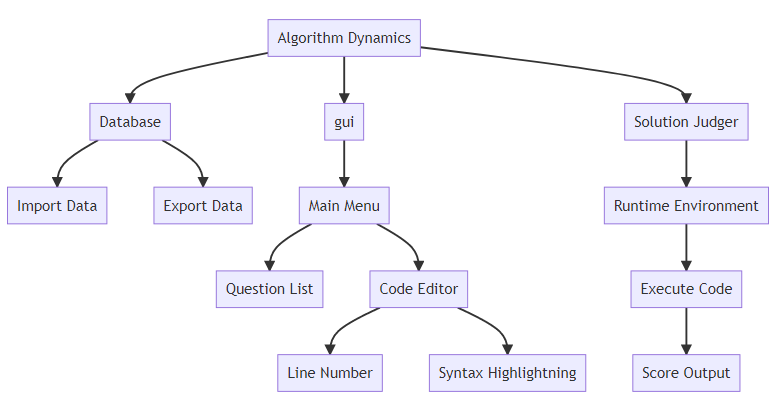
\includegraphics[width=\linewidth]{decomposition-analysis}

\subsection{Thinking concurrently}

When judging the students' solution, many test cases can be executed at the same time to reduce the judging time. The number of parallel judgers needs to be set carefully based on the user's hardware. Running too few test cases concurrently may result in a very long judging time while running too many test cases at the same time may use up computing resources and cause issues.

\section{Interview}

\subsection{Design interview}

\subsubsection{Interview for teachers}

\begin{enumerate}
    \item Do you find your students tend to lose marks on programming questions in exams?
    \item Do you find marking the programming question takes a lot of time and effort?
    \item Compare to the knowledge-based Computer System section, do you find it is more difficult to monitor students' skill level on the Algorithm and Programming section?
    \item Have you ever heard about some online programming platforms?
    \item Have you ever tried some of the online programming platforms?
    \item If yes, what do you think about these platforms? Have you ever considered using them for teaching and training?
    \item Do you think a similar solution can help improve the efficiency of learning and training?
    \item If no, do you think the idea of a software that can mark students' answers on programming questions and provide analysis data can help improve the efficiency of learning and training?
    \item Do you have anything else to add?
\end{enumerate}

Question 1 to 3 is a series of proof-of-concept questions, which I expect my stakeholders to answer `Yes' to all of them. They confirm that the problem I am trying to solve exists and there is a need for such a solution. Question 4 to 5 asks about the teachers' knowledge of existing solutions. Question 6 to 8 ask about their experiences and opinions about these existing solutions, which gives me insights on the problems with existing solutions and how my solution can fit their need better.

\subsubsection{Interview for students}

\begin{enumerate}
    \item Do you find the programming questions difficult?
    \item Do you find yourself lacking efficient practising in algorithm designing and programming?
    \item Have you ever heard about some online programming platforms?
    \item Have you ever tried some of the online programming platforms?
    \item If yes, what do you think about these platforms?
    \item Do you think a similar solution can help you learning and practising?
    \item If no, do you think the idea of software that provides coding questions and marks your answer instantly can help you learn and practice better?
    \item Do you have anything else to add?
\end{enumerate}

Question 1 and 2 are similar proof-of-concept questions to confirm such a problem exists. The following questions ask about students' knowledge of existing solutions. If they have used an existing product before, I ask whether they think it helps. Otherwise, I ask whether they think it will be useful.

\subsection{Conduct the interview}

\subsubsection{Computer Science teacher - Mr Grimwood}

\begin{enumerate}
    \item Do you find your students tend to lose marks on programming questions in exams?

    They do. Many of them don't understand the algorithms.

    \item Do you find marking the programming questions takes a lot of time and effort?

    Yes. Because some students produce partially correct answers, so it takes a lot of time to identify the correct part and award them the corresponding mark. Some students may take completely different approaches which takes a lot of effort to understand and mark them.

    \item Do you find it is more difficult to monitor students' skill level on the Algorithm and Programming section and more difficult to provide sufficient help?

    Yes.

    \item Have you ever heard about some online programming platforms?

    I have. Emm... But I forget the names.

    \item If yes, have you ever tried some of the online programming platforms?

    I have.

    \item If yes, what do you think about these platforms?

    I think the idea is quite interesting and I find them working quite well.

    \item Have you ever considered using them for teaching and practising?

    No. Because most of them require a paid subscription, and their content is more likely to be something like `Learning Python' which is irrelevant to the A Level Computer Science content.

    \item Do you think a similar solution can help improve the efficiency of learning and training?

    Yes. The students can learn at their own pace and they can keep practising by themselves.

    \item Do you have anything else to add?

    No.
\end{enumerate}

Mr Grimwood has several valuable points here. He points out that the `partially correct' answers are the most difficult ones to mark. For my solution, if a student submits a `partially correct' code answer, then its output will certainly not match the expected output. This means my solution might not be able to tell the difference between a `partially correct' answer and an `incorrect' answer. This is a potential limitation I need to watch out for. He also says the price is one of his concerns. My solution will be free and open-source, which will meet his need perfectly. By adding the function to create custom questions and share them with others, users will be able to create and find A Level Computer Science content, or any content easier. It is also a good idea for me to create some A Level Computer Science content that comes with the software to make it easier to use.

\subsubsection{Computer Science student - PCloud}

\begin{enumerate}
    \item Do you find the programming questions difficult?

    I find some of them quite complex and difficult, especially the graph algorithms such as Dijkstra.

    \item Do you find yourself lacking efficient practising in algorithm designing and programming?

    Absolutely. Although I code a lot in my spare time, normal projects are quite different from the exam questions. There are not many past papers and exam-style questions for practising, so I usually don't feel confident of those questions.

    \item Have you ever heard about some online programming platforms?

    Yes. Such as AcWing, LeetCode, and TopCoder.

    \item Have you ever tried some of the online programming platforms?

    Yes. I am an active user of AcWing.

    \item If yes, what do you think about these platforms?

    I enjoy the experience. They can provide instant feedback for my submissions. It provides very strong positive feedback when I solve a new question. I find myself learning faster and more efficiently with such platforms.

    \item Do you think a similar solution can help you learning and practising?

    Absolutely. The existing platforms do not provide A Level related content. So if a software solution can be altered for A Level Computer Science course, that will help a lot.

    \item (*) How do you think it should be optimized for A Level CS content?

    You can add past exam questions practising. Add a timed practice mode will be helpful.

    \item Do you have anything else to add?

    No.
\end{enumerate}

PCloud confirms that such a solution will help him learning and practising more efficiently. The instant feedback of whether he gets the question correctly is very important to him. Instead of sending the user's submission to a remote server, my solution should judge the user's answer on their computer. This can avoid the instabilities caused by the remote server's availability and the network connection. He also gives me some good ideas about the content. I can add past exam questions for users to do timed practice, which enables users to practice algorithms and exam techniques at the same time.

\subsubsection{Computer Science student - Timofei}

\begin{enumerate}

    \item Do you find the programming questions difficult?

    Yes. I generally lose marks because of some careless syntax mistakes I made.

    \item Do you find yourself lacking efficient practising in algorithm designing and programming?

    Yes. I find I cannot find many materials to practice.

    \item Have you ever heard about some online programming platforms?

    Codewar. Something like that.

    \item Have you ever tried some of the online programming platforms?

    Yes.

    \item If yes, what do you think about these platforms?

    I think they are quite helpful. But I find their marking is too specific, if I get a single character wrong in my output, it gets marked incorrect.

    \item Do you think a similar solution can help you learning and practising?

    Yes.

    \item Do you have anything else to add?

    No.

\end{enumerate}

Timofei points out that the marking system in existing products is not very sensible. This may be a potential limitation of my solution as well. It is easy to directly compare the users' output and the expected output. But if they are different, it is difficult to figure out whether that difference is caused by a wrong code solution or just some formatting error. I can partially solve this by allowing the users to pre-test their code against examples before formal submissions, so they can check the output format.

\section{Research}

There are many coding training websites on the market, most of them share a similar idea, so I will investigate two of the most popular ones.

\begin{itemize}
    \item LeetCode
    \item Codeforces
\end{itemize}

\subsection{LeetCode}

\href{https://leetcode.com/}{LeetCode} is a platform for interview coding training, many large companies (Google, Facebook, ...) use it as a part of their interview.

LeetCode provides a database containing more than 1000 coding questions.

\subsubsection{Main coding layout}
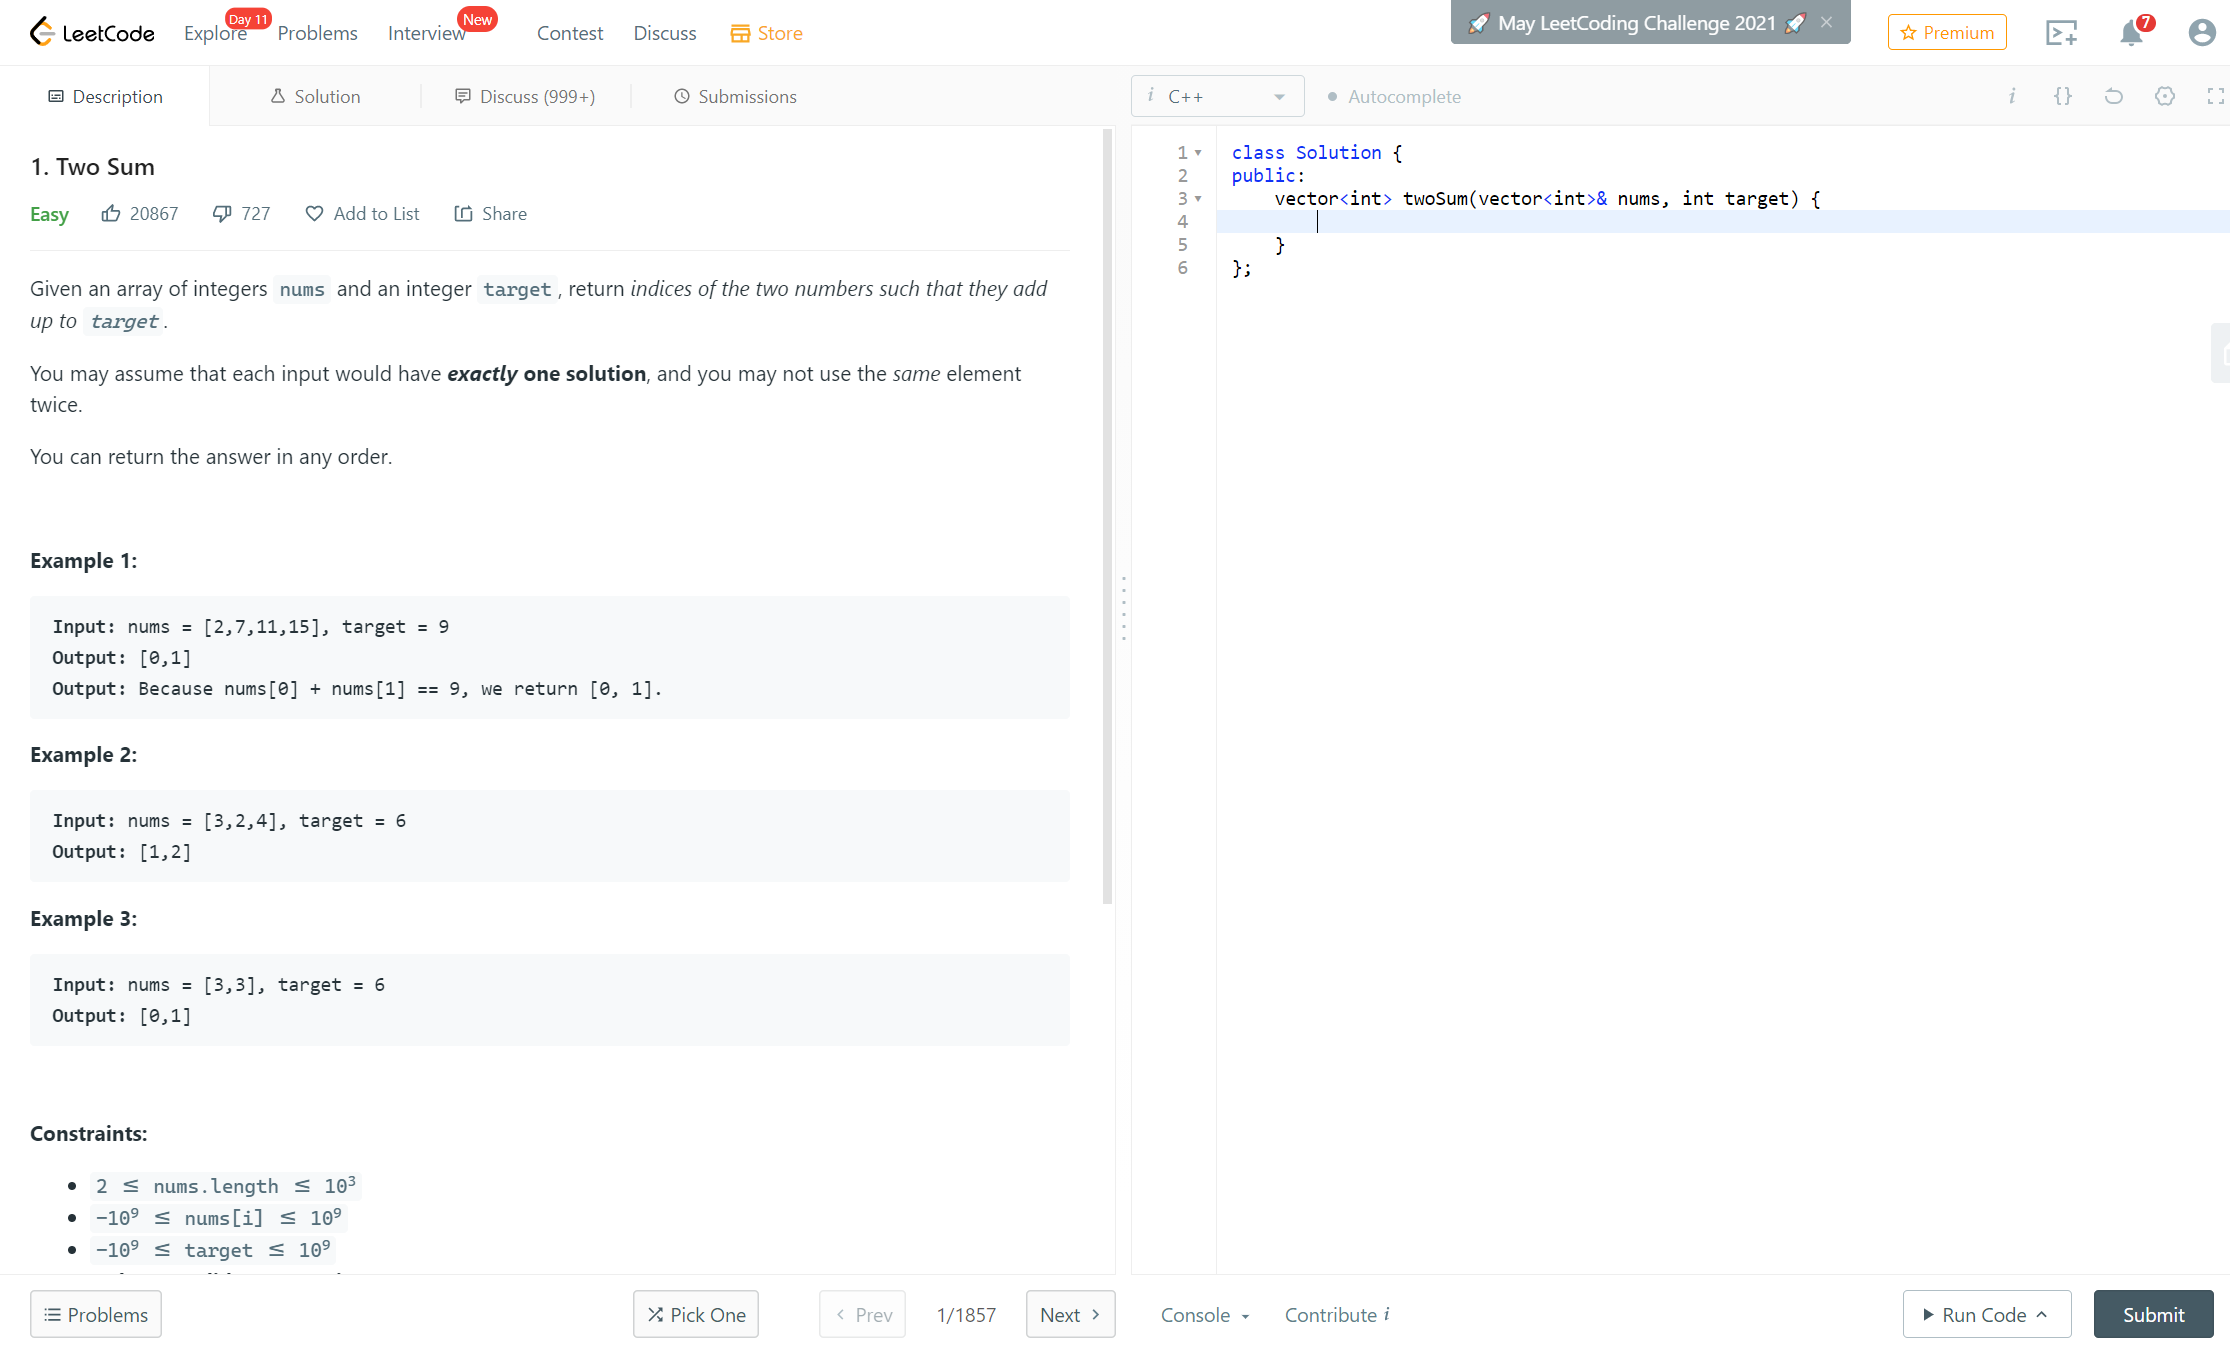
\includegraphics[width=\linewidth]{Two-Sum-LeetCode-Coding}

This is LeetCode's main coding area. The user's screen is split into two parts - the question section and the code editor for inputting answers. Users can drag the splitter in the middle to adjust the size of each section.

The question section contains 4 tabs, `Description' tab displays the content of the question. `Solution' tab displays the solutions from the community. `Discuss' tab displays the discussions in the community. `Submission' tab lists the user's previous submissions. Since I am not adding social functions in my solution, I will ignore the `Solution' and `Discuss' tabs. Under the `Description' tab, LeetCode provides the context of the question, followed by 3 examples, and constraints for this question. The examples allow the user to run and check their solution before formal submission for marking, this can help them avoid silly mistakes. My solution should also provide similar examples for each question. Under the `Submission' tab, LeetCode records every history submission, so the user can revise old questions more efficiently. My solution should provide a similar function as well.

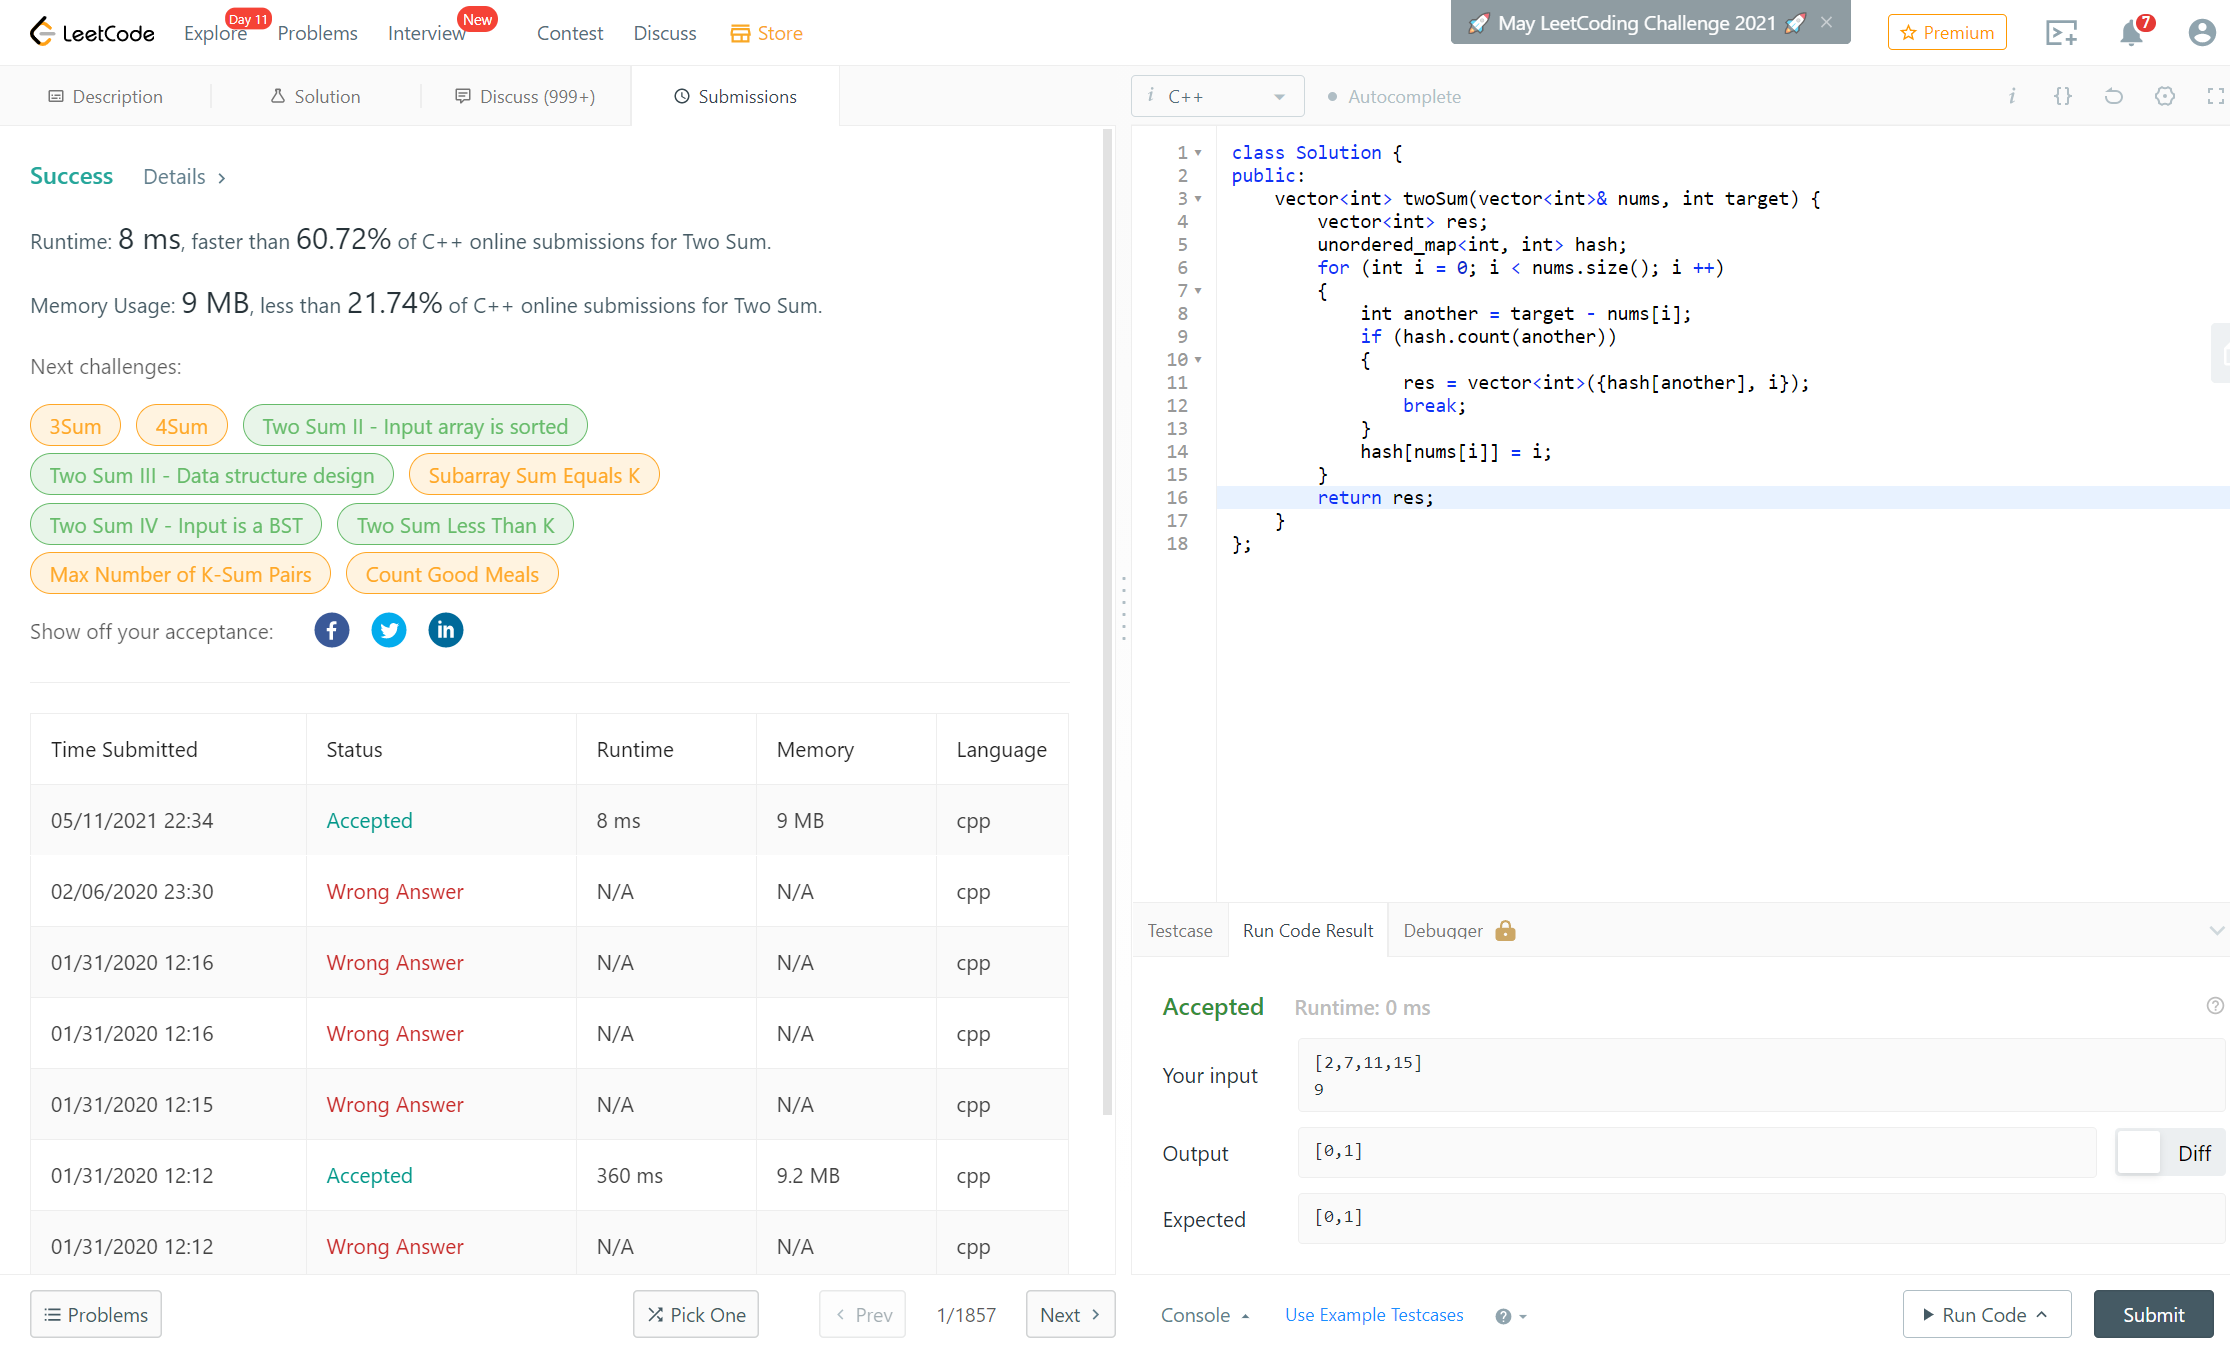
\includegraphics[width=\linewidth]{Two-Sum-LeetCode-Submission}

The code editor provides line number and syntax highlighting functions. User can change their programming language with a drop-down box. LeetCode supports all mainstream programming languages. My solution should be able to support multiple programming languages as well, which allows students with different backgrounds to use it easily.

On the button, the user can `Run Code' to test their code against the examples before submission, and then click the `Submit' button to submit their solution formally.

The split view design is clean and handy. The user can see the question and write their solution on the same page without switching between different windows. The design of examples and the `Run Code' button is useful as well. I can refer to LeetCode's coding layout when designing my solution's interface.

\subsubsection{Question database}

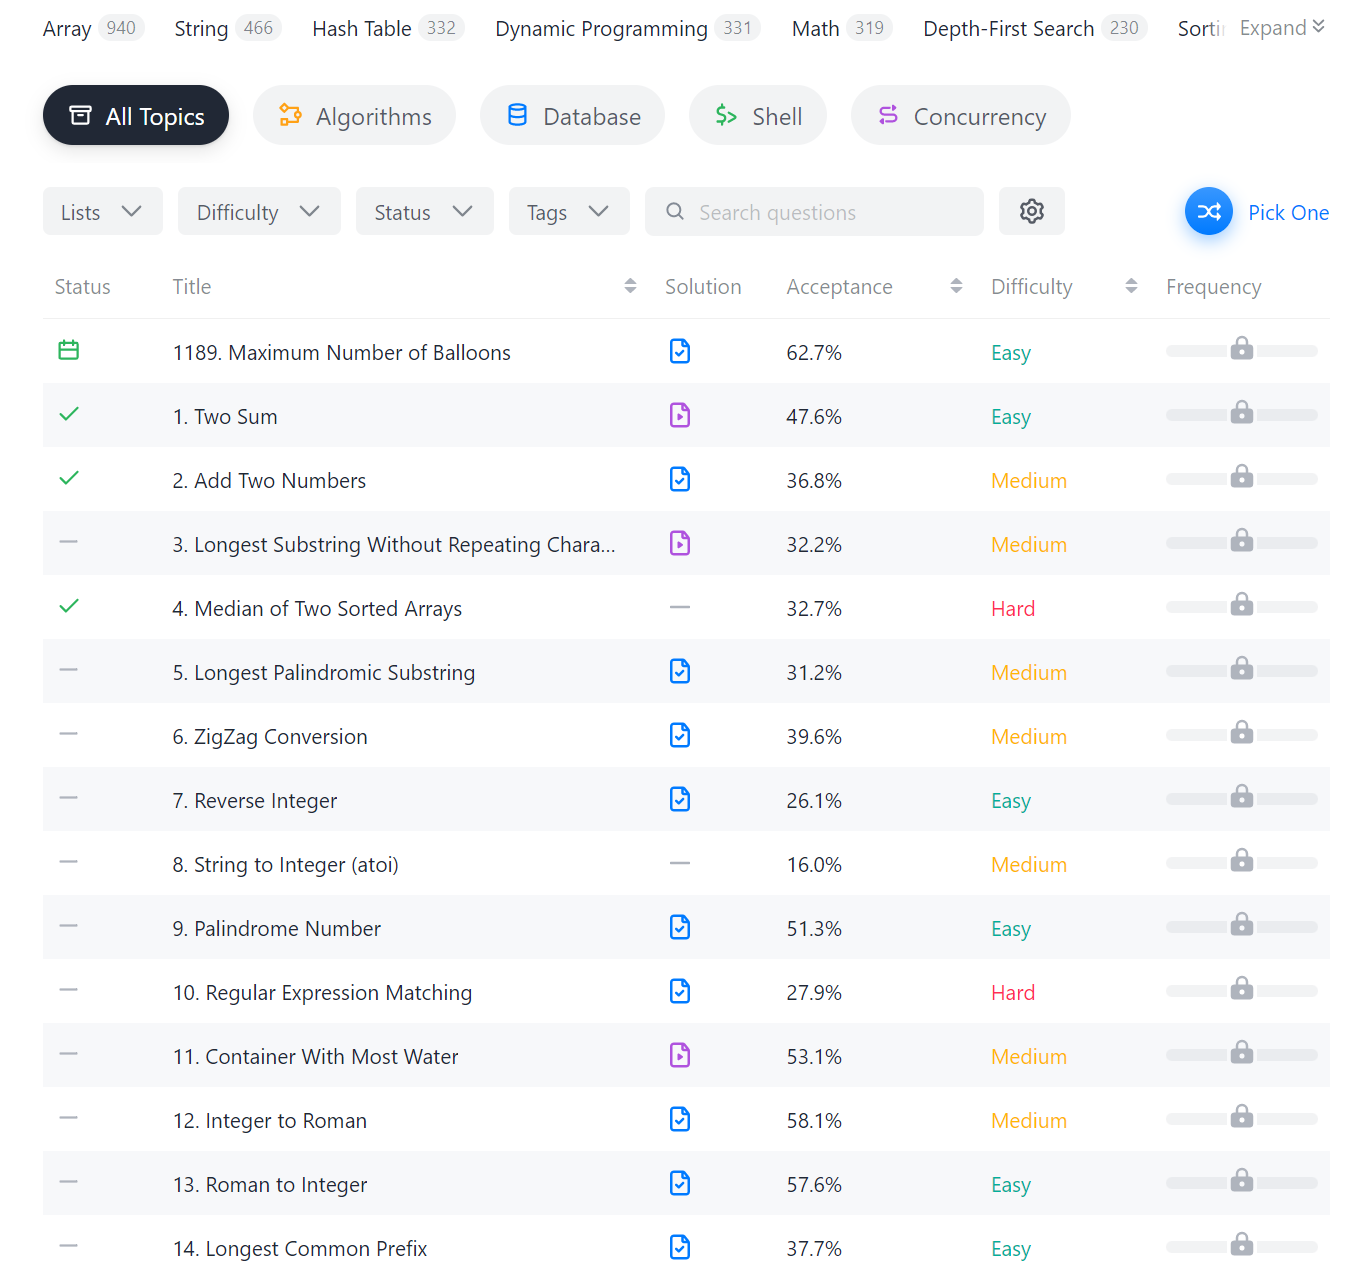
\includegraphics[width=\linewidth]{LeetCode-Problems}

Every question in LeetCode has many different attributes (Lists, Difficulty, Status, Tags, Title, Acceptance), so it is very easy for a user to find a suitable question to practice. My solution can similarly organize the question database and provide a corresponding query interface for a better user experience. The `Pick One' button on the top right is a very handy feature as well. Users can simply click that button to start working on a quick random question. The idea of `a list of questions' is great. Users can organize a series of questions to practice and share.

\subsubsection{Pricing}

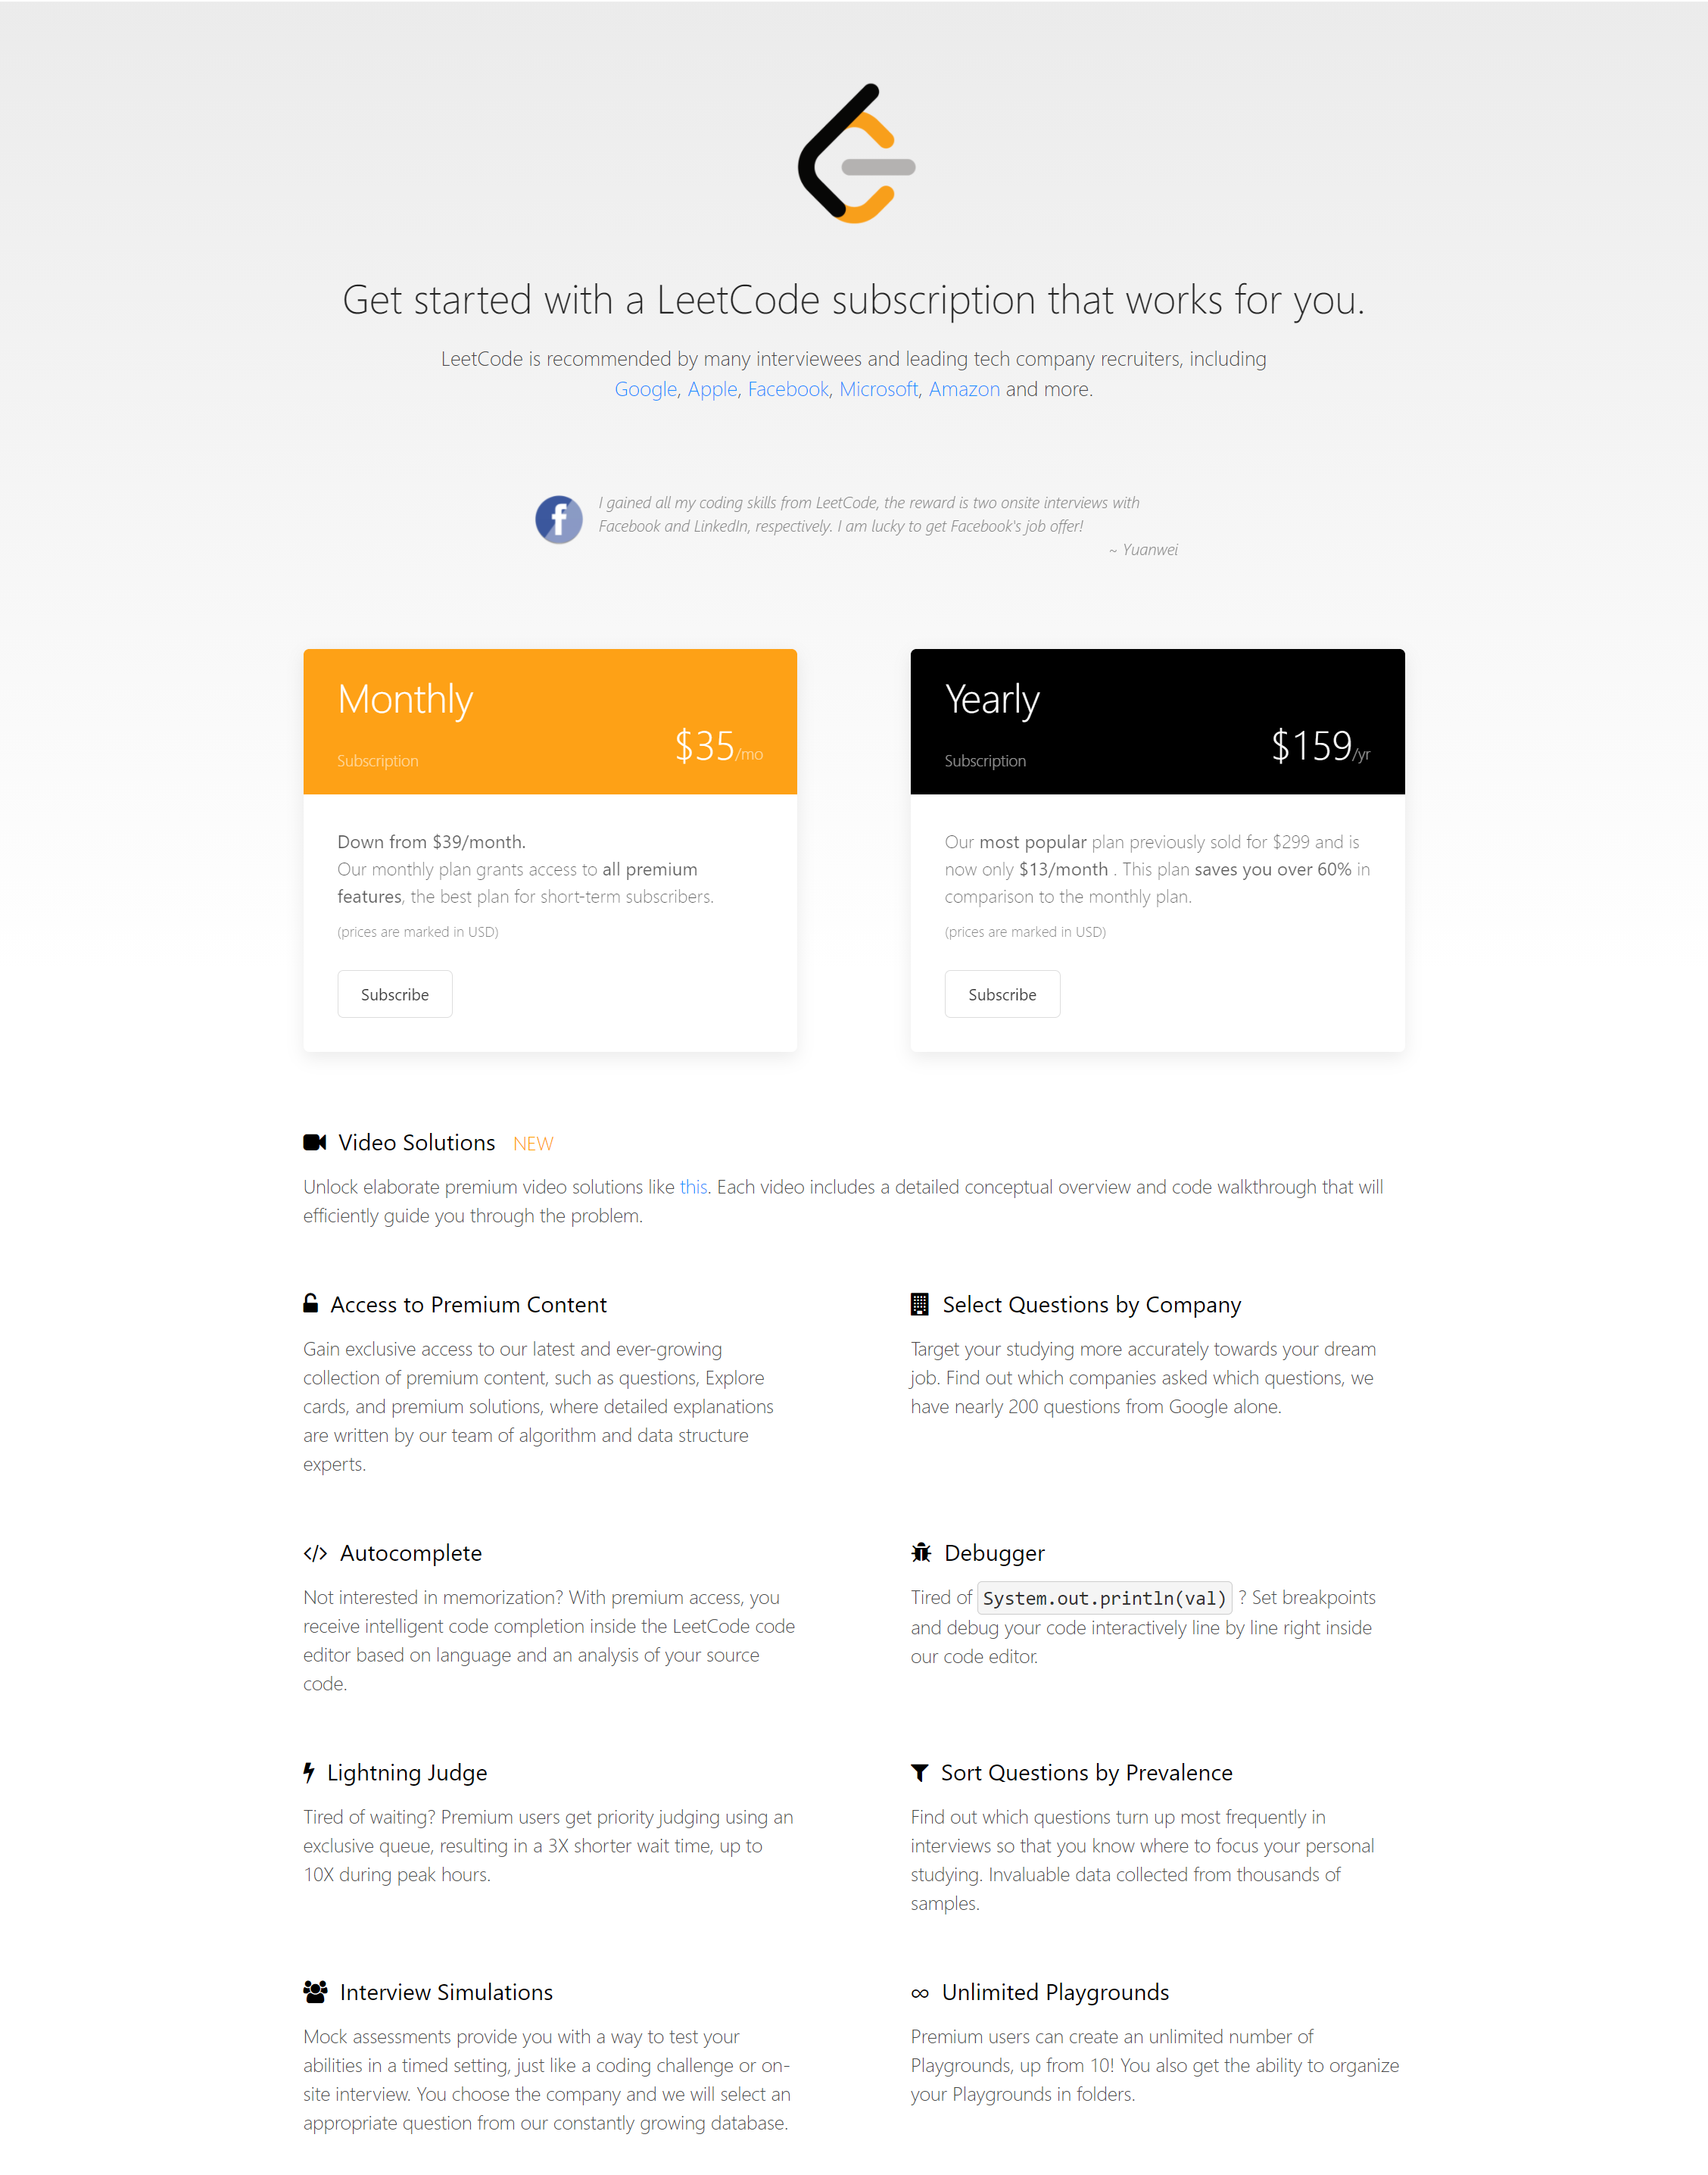
\includegraphics[width=\linewidth]{LeetCode-Premium}

The basic functions of LeetCode are free to use for all users and it charges a fee for premium subscriptions. The premium subscription provides a larger question database, better code editor, faster judger, and more.

\subsubsection{Analysis}

LeetCode is a fully web-based solution, which means it works on any device. However, it also means you will not be able to use it without a stable Internet connection. I decide to make my solution a desktop application since most students practice coding with a computer. It also save me a lot of cost from running and maintaining a server. LeetCode runs a large community for users to discuss questions with each other. I am not adding such a function to my solution. Teachers and students can use existing platforms they have been familiar with, it is unnecessary for me to develop a new platform and for the users to migrate from mature solutions. LeetCode has an easy-to-use graphical interface, which is important so new users can get their hands on very easily.

LeetCode does not support custom questions or any functions for educators. It is mainly designed for self-learners. My solution is designed for school use, so it must support functions like custom questions, custom assignments, statistics data visualizations. LeetCode charges a subscription fee for essential functions. My solution will be free and open-source so everyone can benefit from it.

\subsection{Codeforces}

Codeforces is a competitive coding platform, it is mainly used by people to the held coding competition.

\subsubsection{Main question layout}

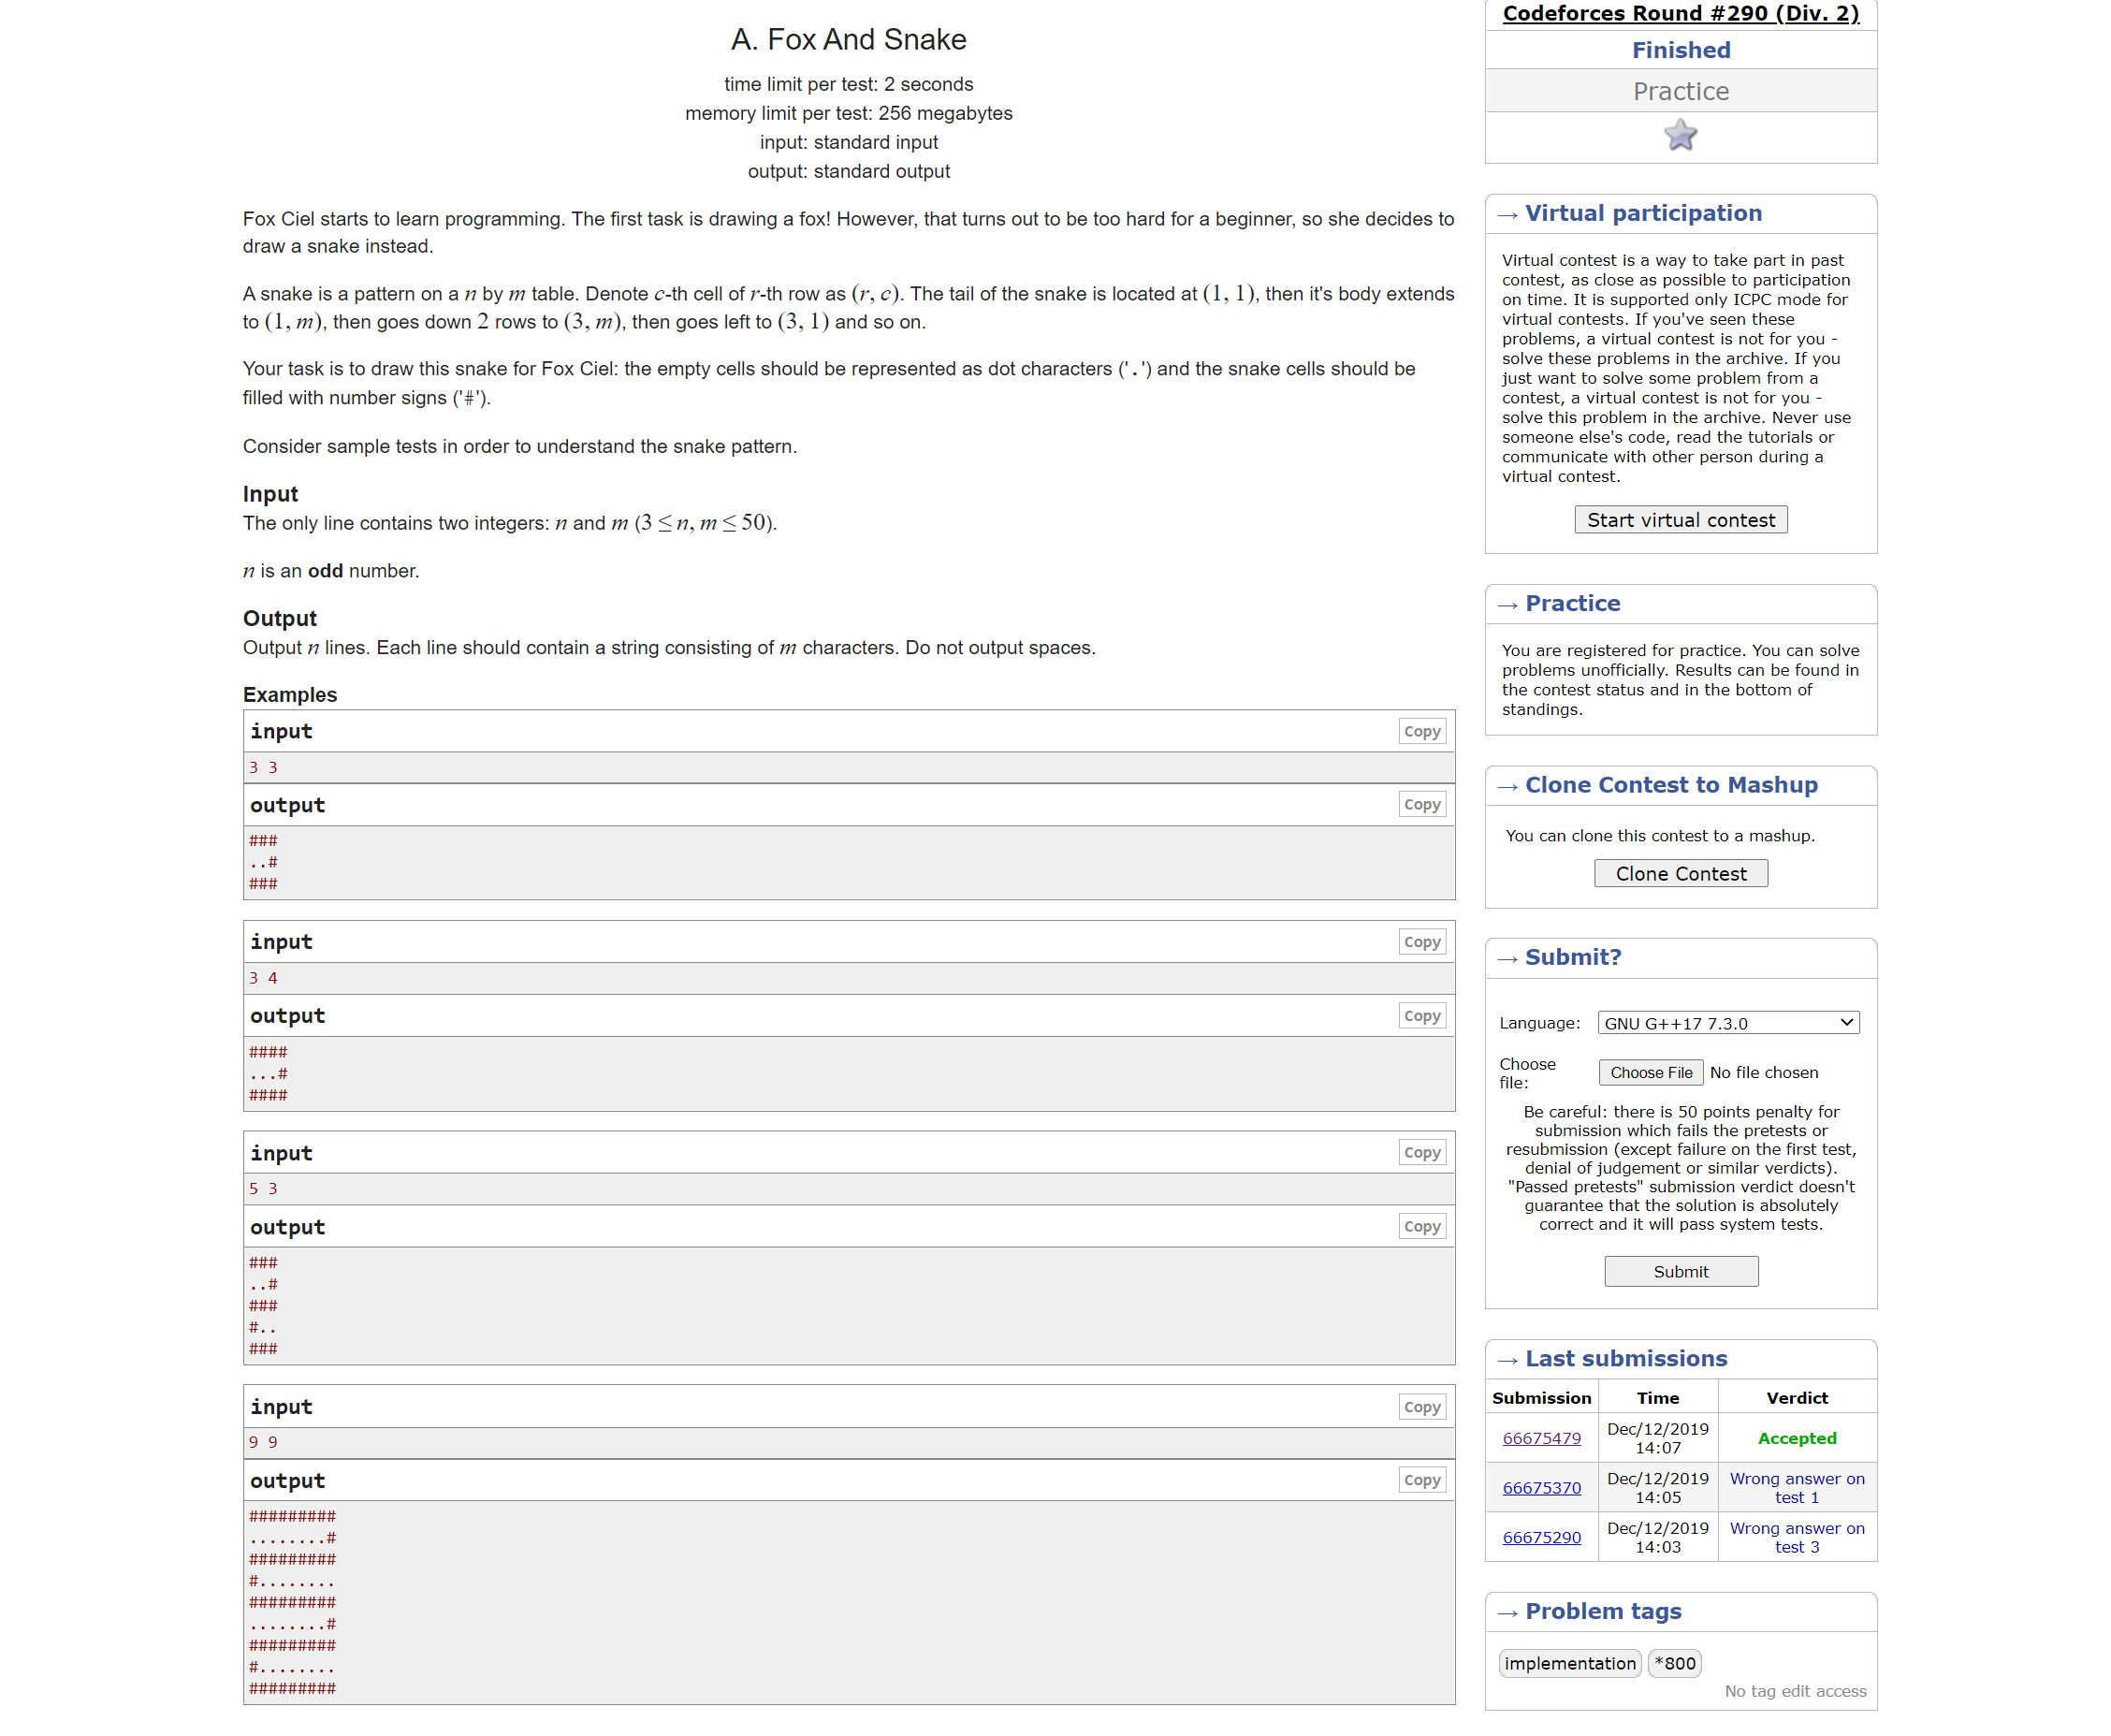
\includegraphics[width=\linewidth]{Problem-A-Codeforces}

The questions and the examples take up nearly all the spaces on the question page. There is no online editor or online runtime environment provided. Users are expected to write and test their code in their IDEs and only submit the solution for judging. Custom IDEs may be more powerful than a built-in one. My solution will provide an editor, it is much more convenient to use. Even if a user decides to use his environment, he can paste his code into the editor for submission. It sets the time and memory limits for users' submissions, if a piece of code takes too long to run, or takes up too much memory while running, it will be terminated and marked wrong.

\subsubsection{Submission}

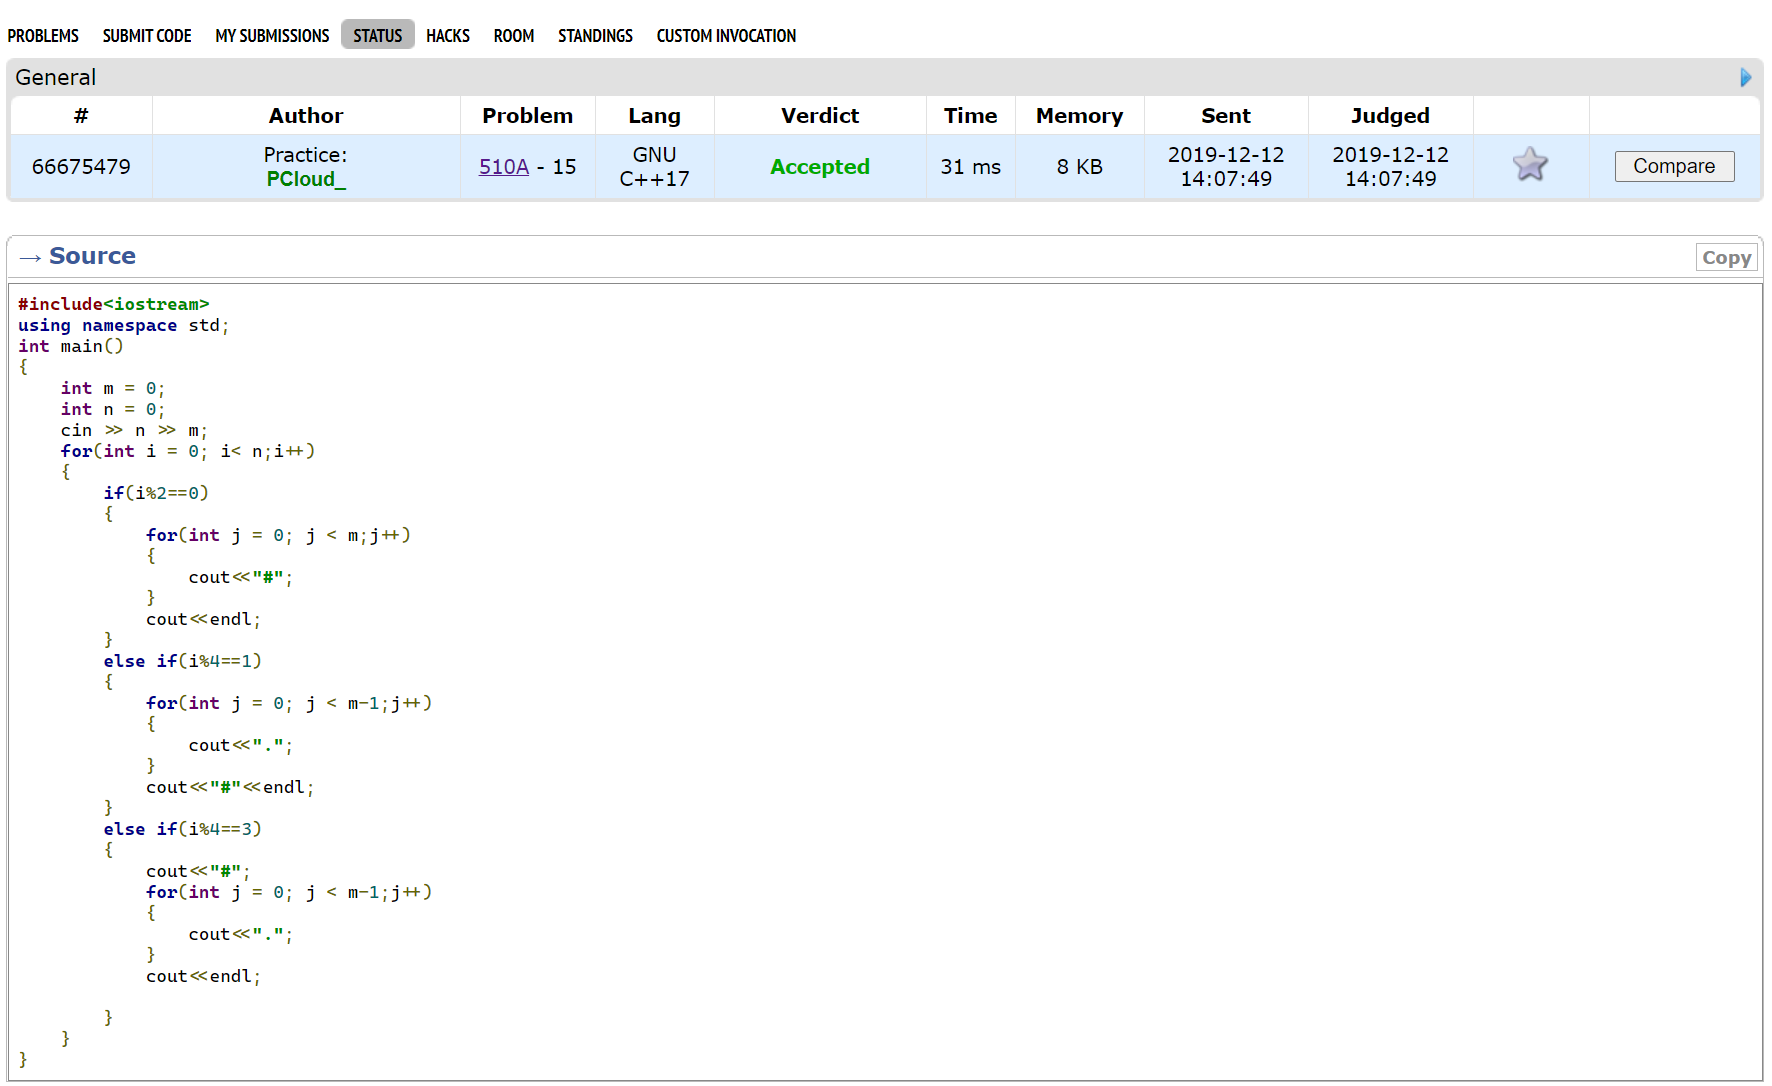
\includegraphics[width=\linewidth]{Submission-66675479-Codeforces}

When the user submits the code, the code enters a queue waiting for judging, then the user can look up their result. Users can check their source code, performance stats, and more importantly, when they have not passed all test cases, they can see what they have got wrong. The judgment protocol provides detailed information about each test case, so users can debug easily.

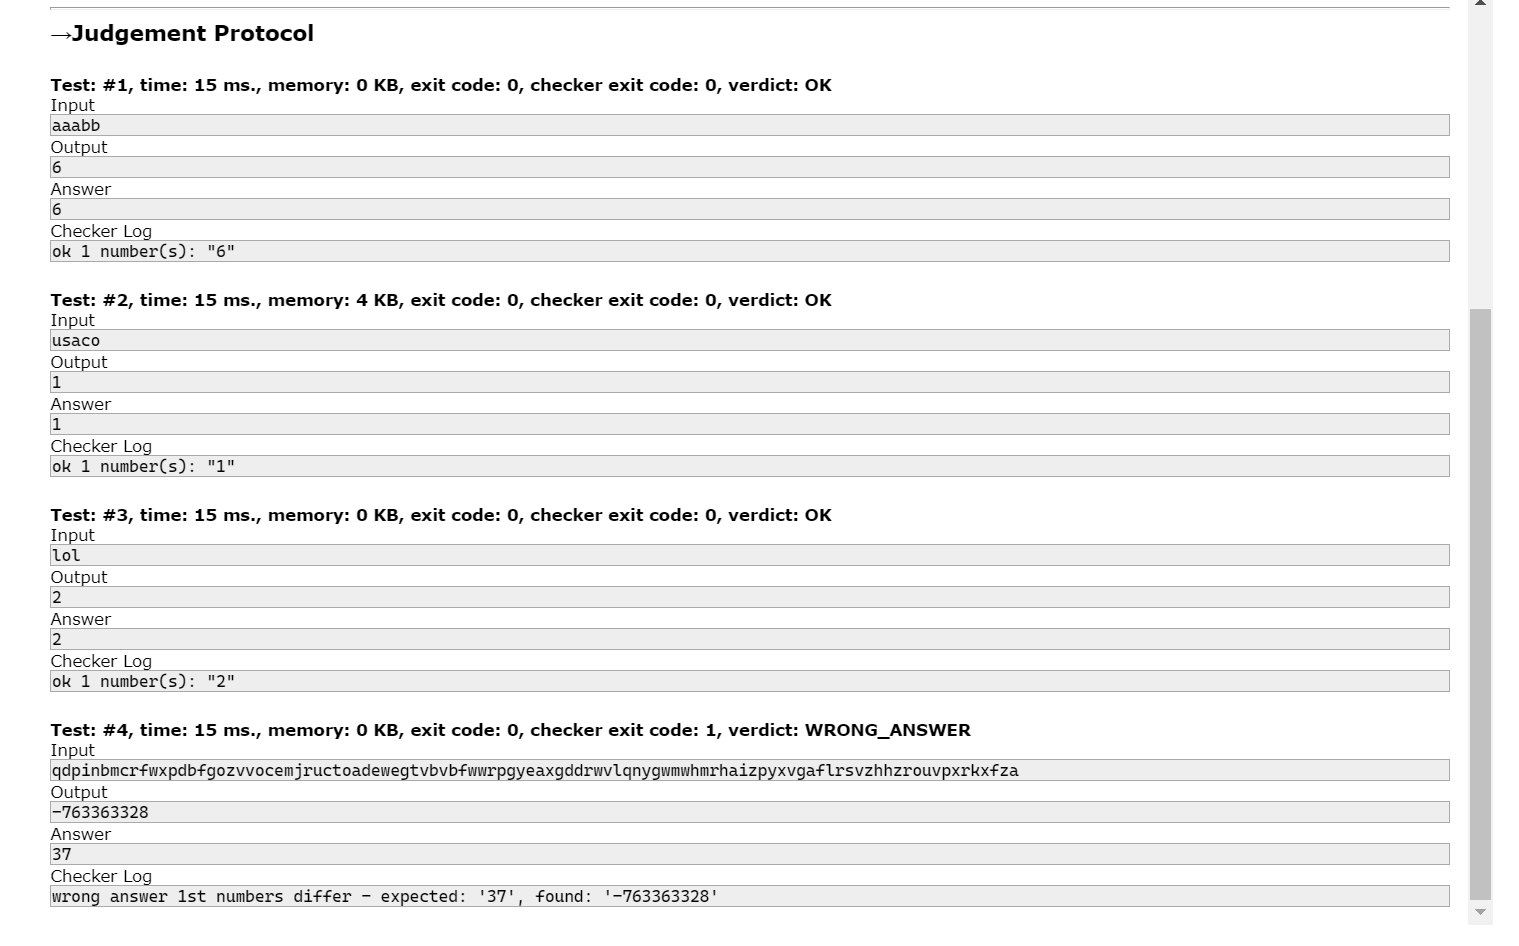
\includegraphics[width=\linewidth]{Judgement-Protocol-Codeforces}

\subsubsection{Analysis}

Codeforces is optimized for coding competition, so it has a lightweight and complex interface for better performance. It is completely free to use. Users can create their questions but it is very complicated to do so. My solution needs to enable users without experience to create questions easily. There is no function for education - there is no way for a teacher to `create a class' and monitor his students. Codeforces is an online platform, so it also works across all devices and requires an Internet connection. Users have to use their IDEs to write and debug their code. Codeforces sends all submissions to a central `judging queue' for marking. My solution will mark all submissions locally, which makes judging a lot faster and save me from running a server. By limiting time and space allowance, Codeforces effectively prevents malicious code from running.

\section{Features}

A useful homepage interface with shortcuts to different functions in the software and other resources outside the software. This allows the user to get into practising faster and makes the software easy to use. Details about the design of the homepage will be discussed in the Design chapter.

A problem database with a graphical user interface. The GUI will have a search box and several drop-down menus for the user to input information to search for a problem. This provides the user with a simple way to find the problems they want, and it also ensures the users can manage and backup the data easily.

An interface for users to create new problems and share them with others. This interface will have multiple text fields for the user to input the descriptions to the problem, the expected input/output data. Then the problem is saved to the database and can be exported to a JSON file allowing the user to share it with others. Users can also create a `list' of problems and export the entire list into a JSON file and share it with others. This enables teachers to create custom problems and share them with the students. It is a core feature that differentiates my solution from the existing ones.

An interface for teachers to create assignments. An assignment is a `list' of problems with some extra data, such as the due date and total mark. It can be exported to a JSON file and share with students. The student's submission will be exported into a JSON file as well and can be sent back to the teacher. The solution will also integrate with the assignment function in Microsoft Teams for Education, which makes it even easier to do. The students' submissions will be automatically marked by the software and detailed data will be provided to the teacher. A simple data analysis interface will be provided to the teacher so they can have a brief look at the result. The teacher can also export the data into a CSV file so they can import it to their school system or analysis it with professional software. This automates the entire process from creating assignments, distribute assignments, collecting assignments, and marking assignments. Teachers will have more time analysis the student's performance and provide corresponding help timely. It is a core feature that differentiates my solution from the existing ones.

An interface displaying the problem and the code editor. The solution provides a `Run Code' button for the student to pre-run their code before submission, a `Submit' button for the student to submit their code. This allows the students to read the question and write their code solution without switch between different windows. The `Run Code' function also makes it easier to debug their code.

A playground with a code editor and runtime environment. This allows the software to be used in class teaching as well, the students can experiment with different algorithms and programming languages in the playground easily.

A settings page contains all the setting options for the software. Users can adjust settings such as their preferred programming language, syntax highlighting settings, colour themes, and so on. This allows the users to customize the software to fit their needs and allows users with different backgrounds to use it without issues.

\section{Limitations}

The software will be written in C\# instead of web-based which means extra software needs to be downloaded by the user. I plan to use .NET 5 runtime and WinUI 3 library for my solution, so only the Windows 10 1809 or newer Windows operating systems will be supported. This should not cause many compatibility issues since most school computers are running the required version of the operating system. Downloading an extra software is inconvenient and may violate the IT security policy of some schools.

The judger can only accept code submission in limited programming languages and the user may require to configure their runtime environment. Creating a compiler for `OCR Pseudocode Programming Language' is too complex for this project. I will attempt to allow the user to add their preferred programming language and write documentation for them to make the process easier.

Unlike LeetCode, there are no Discussion pages for users to discuss questions because it is a desktop program instead of a web one. But this is not a big problem, students and teachers should use an existing product such as Microsoft Teams which has very good support in sharing code snippets. It is unnecessary to rebuild the wheel.

Distribute the questions and assignments is still something inconvenient. Currently, distributing questions and assignments requires the teacher to first export the questions and assignments, then send them to the students through email or file-sharing platforms. When the students finish working, they need to send their results back through email or other apps. I have attempted to integrate the file-sharing function with the existing platform - the Microsoft Teams Assignment function. \sout{But unfortunately, the Graph API required for this operation is still in beta version, which means it can only be tested in the development environment and cannot be used in production. So for now, the users still have to use this inconvenient way to share questions and submissions. But in the future, the integration with some existing platforms may improve the experience.} (Update: the Microsoft Teams API is out of beta, now it is possible to integrate with it)

There are no good ways to maintain and distribute a large question database. Computer Science teachers are required to maintain a database for their students. But this is difficult work. Creating good test cases is much time consuming than writing a mark scheme, it is very likely for a wrong solution to pass the judging if the test cases are not good enough. It relies on the teacher who creates the questions to consider everything clearly to minimize its impact.

The judger can only simply compare the students' output with the expected output if there is a format error such as trailing space and extra newline in their output, which will not be considered as a mistake in a real exam, will be marked as a wrong answer by the judger. So students may need to spend extra time debugging their output format. It cannot judge ``partially correct'' answers as well. It does not care which line did the student get correct or wrong, if the final output doesn't match, the submission will be marked wrong.

\section{Hardware and software requirements}

\begin{tabulary}{\linewidth}{|L|L|}
    \hline
    Hardware and software requirements & Justification \\
    \hline
    Standard mouse, keyboard, and monitor. & Standard I/O devices are required for the user to interact with the software. Users need a mouse to navigate around different menus and pages, they need to use a keyboard to input their code solutions and use a monitor to get the output from the software. \\
    \hline
    Operating system: Windows 10 (1809 or later), Windows 11. & The software is designed with the WinUI 3 library and .Net 5 runtimes, which require such an operating system to run. \\
    \hline
    x86 64-bit CPU (Intel / AMD architecture) with 2 or more cores and 1 GHz or higher clock speed. & A modern CPU is required for the software. 1 core will be used to run the main program and at least 1 spare core is required for the judger to judge the submitted code. A clock speed higher than 1 GHz is required to ensure the software is running smoothly. \\
    \hline
    1GB free memory or more. & Around 512MB RAM is required to run the software, and another 512MB RAM is required for the judger to judge the submissions. \\
    \hline
    256MB free disk space or more. & 256MB free disk space is required to store and run the program itself, the user may need extra disk space to store extra cache data and the database. \\
    \hline
    A modern dedicated or integrated graphics card. & The software has very little graphical demand, if the user's graphics card can run their operation system, it should be able to handle software as well. \\
    \hline
\end{tabulary}

\section{Success criteria}

\begin{tabulary}{\linewidth}{|L|L|}
    \hline
    Criteria & Justification\\
    \hline
    Users can use different links, menus, and buttons to navigate around the software easily. & This ensures the program is easy to use and allows the user to find the function they want to use quickly.\\
    \hline
    Users can use different drop-down menus and the search box to find a problem from the problem database. & This allows users to search for questions easily in the database.\\
    \hline
    Users can add new questions to the database. & This allows teachers to create new algorithm problems.\\
    \hline
    Correctly validate the new questions before adding them to the database. & Make sure correct data is input and prevent SQL injection.\\
    \hline
    Users can create lists of questions. & This allows teachers to organize problems better by creating lists to manage them.\\
    \hline
    Users can create assignments. & This allows teachers to create new assignments for their students.\\
    \hline
    Users can export/import questions, lists, and assignments from/to their problem database. & This allows the users to share questions and data with others easily.\\
    \hline
    Users can work on a problem and their submissions can be automatically marked by the judger. & This allows the users to practice and get feedback on the software.\\
    \hline
    Users can create submissions for assignments and export them into a file. & This allows the students to complete and hand in assignments easily.\\
    \hline
    Correctly access and interact with the Microsoft Teams API & Allowing teachers and students to manage assignments through Microsoft Teams.\\
    \hline
    The software can mark the assignments automatically. & This automates the marking process and reduces teachers' work.\\
    \hline
    The software can perform simple data analysis to the assignments data. & This provides teachers with an overview of student's performance on their assignments and allowing them to help their students better.\\
    \hline
    Users can export the assignment data to CSV files. & This allows the teachers to use advanced data analysis tools and import the data into their school system.\\
    \hline
    Users can use the playground to test any code. & This allows the users to experiment with new algorithms and programming languages and allows the software to be used in class teaching.\\
    \hline
\end{tabulary}

\begin{tabulary}{\linewidth}{|L|L|}
    \hline
    Users can customize the software. & This allows users to work in their favourite environment and makes the solution suitable to users with different backgrounds.\\
    \hline
    Split the core functions and class into a core library. & Allowing easier maintenance. \\
    \hline
    Using sensible variable names and add comments to each function. & Makes the code easy to understand and make maintenance easier.\\
    \hline
    Create CI/CD pipelines to build and deploy the application automatically. & It allows the software to be tested and deployed automatically so users always receive the latest features and security updates.\\
    \hline
    Unit tests with coverage higher than 90\%. & It makes sure all code is well tested. \\
    \hline
\end{tabulary}

All the success criteria will first be tested through the unit tests created during the development. Then they will be tested and improved by me during the Alpha Testing stage. Finally, they will be tested by the stakeholders in the Beta Testing stage, and the evaluation will be based on their user experience and opinions.

\chapter{Design}
\section{Decomposition}

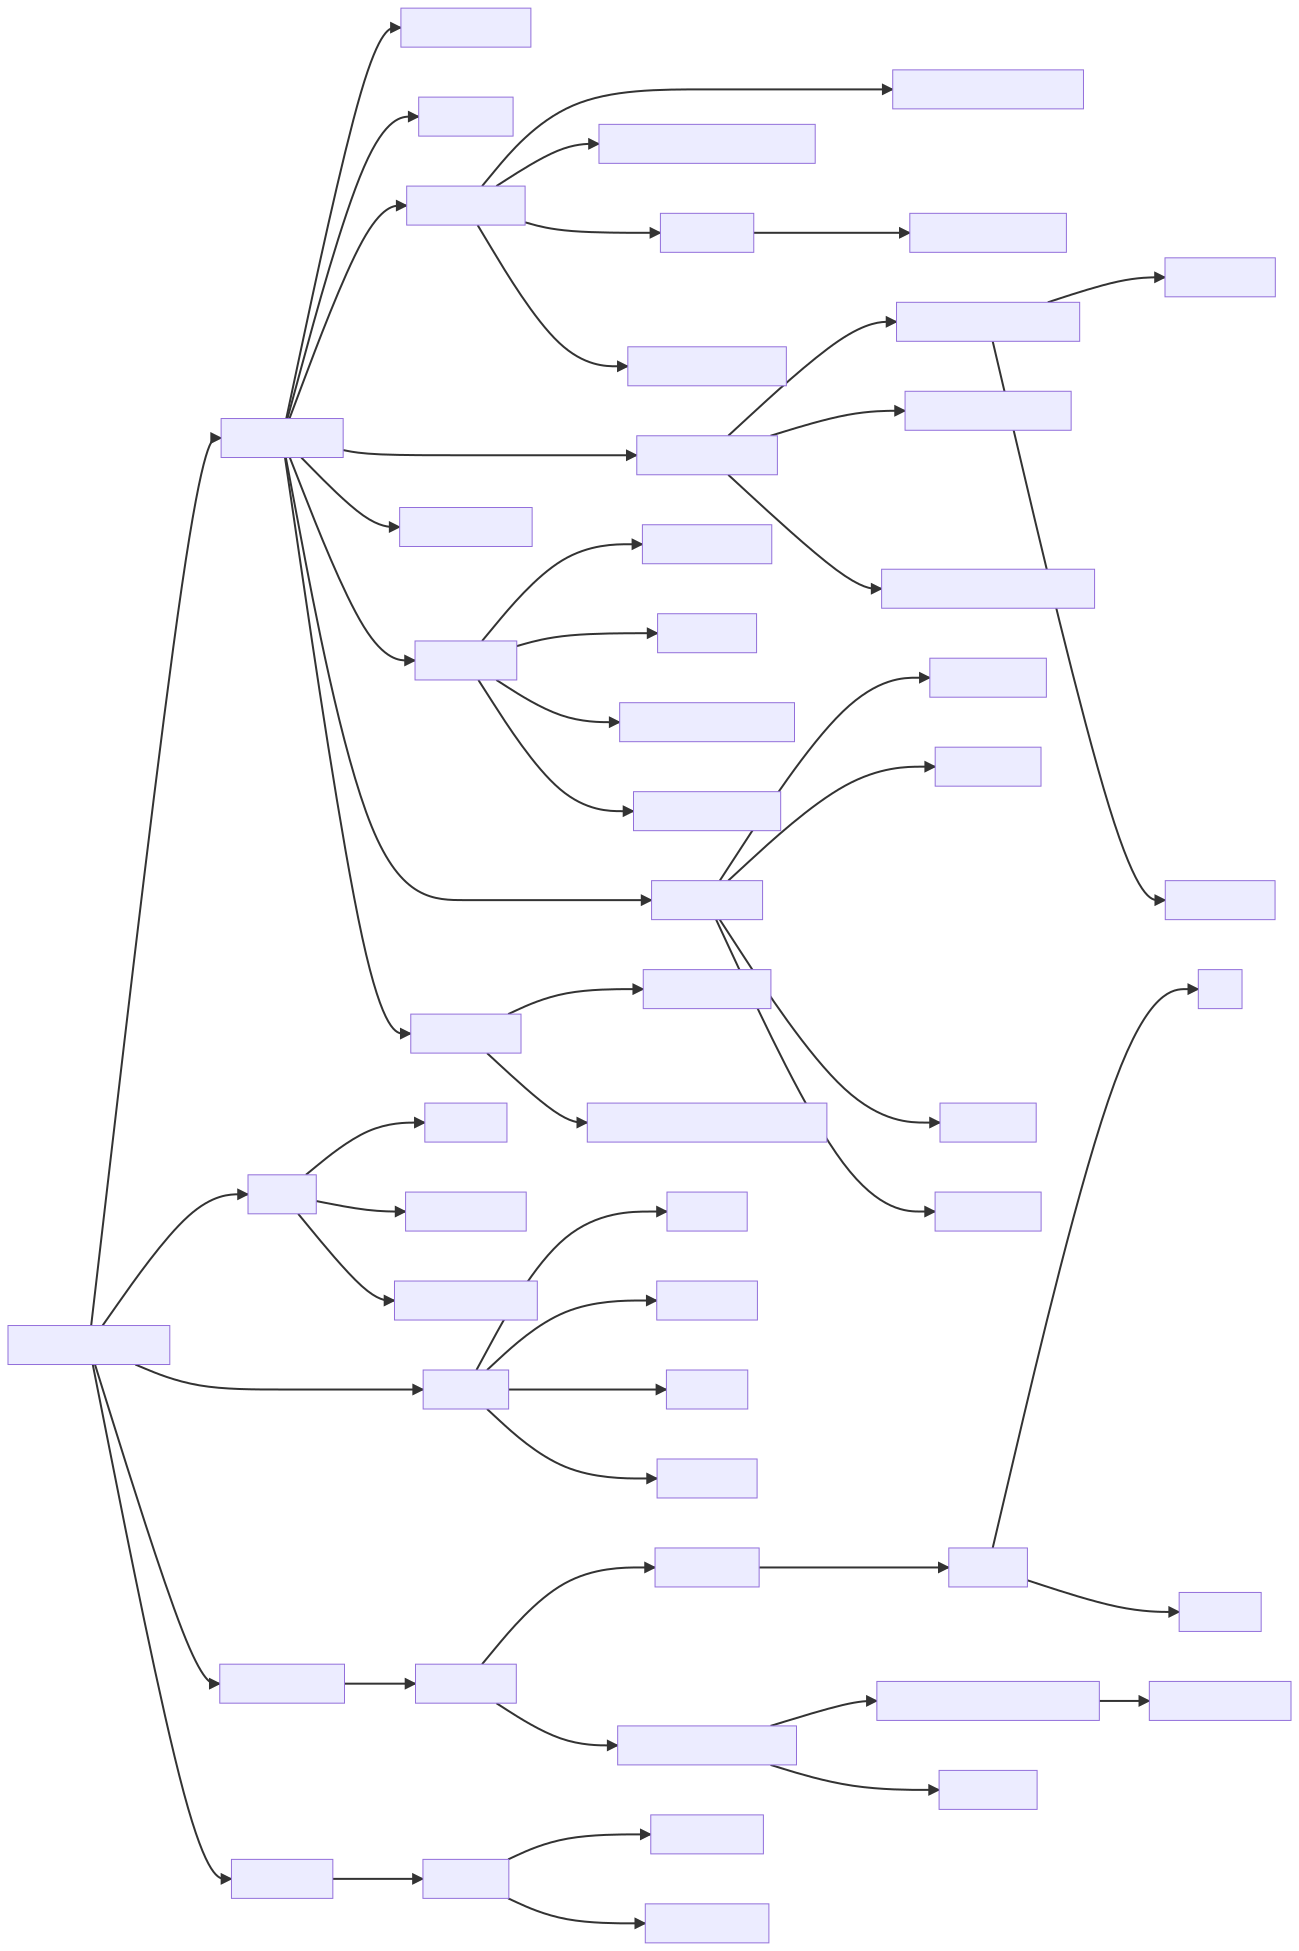
\includepdf[pages=-]{graphs/decomposition-design.pdf}

\subsection{NavigationView}

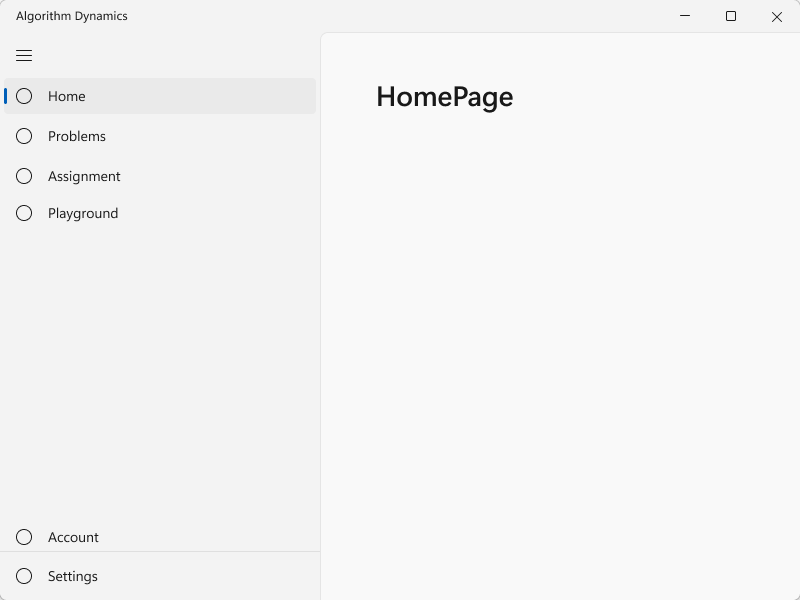
\includegraphics[width=\textwidth, height=\textheight, keepaspectratio]{NavigationView-Design}

The Navigation View provides a global menu for the user to navigate between different pages in the software. There are six tabs in the navigation view, ``Home'', ``Problems'', ``Assignments'', ``Playground'', ``Account'', ``Settings''. By clicking on different tab, the main frame will display the corresponding page. The current selected tab will be highlighted.

\subsubsection{Usability Feature}

The entire NavigationView is a usability feature. Users can always look it up by clicking the top left button. They will be able to know where they are and navigate to other pages by one click, which makes the program easier to use.

\subsubsection{Validation}

There are only buttons in the NavigationView for the user to click, so only valid actions can be taken, no further data validation is required.

\subsection{HomePage}

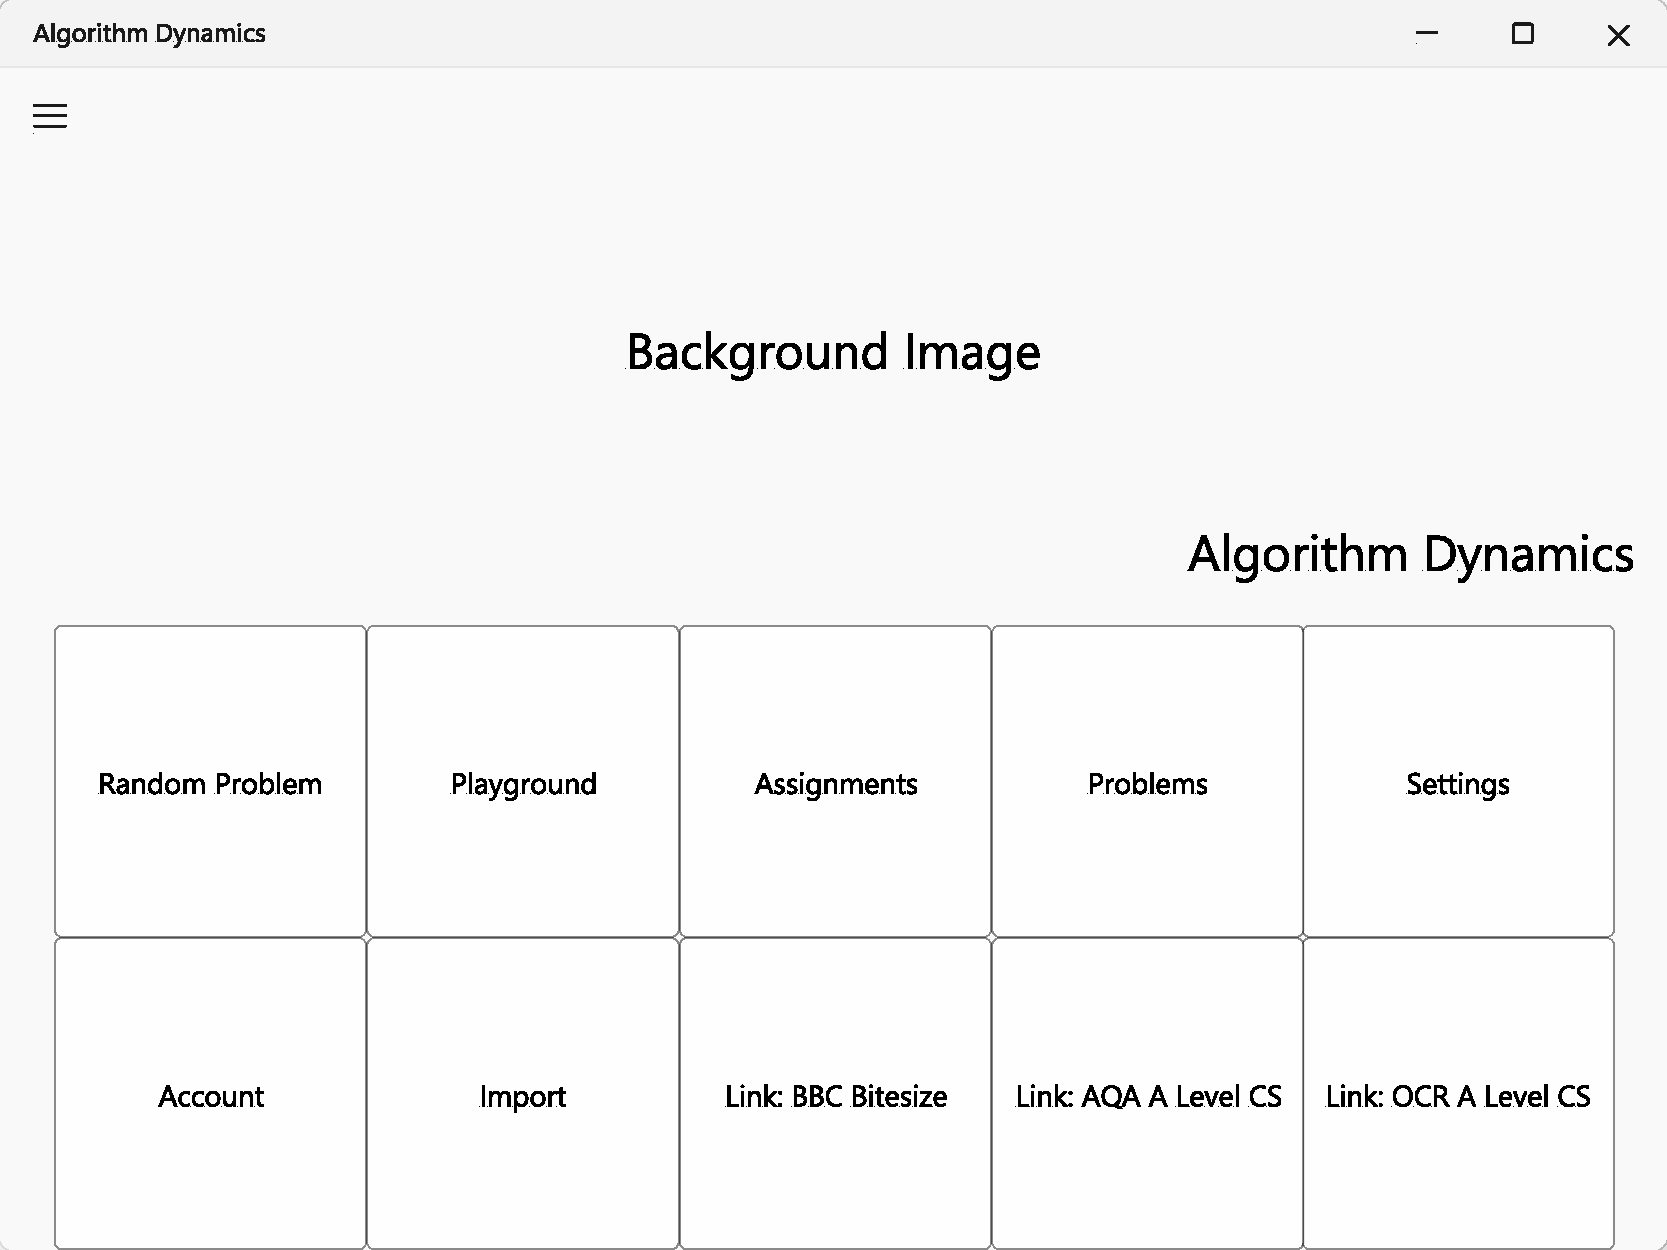
\includegraphics[width=\textwidth, height=\textheight, keepaspectratio]{HomePage-Design}

On the top of the HomePage, there will be a beautiful background image under the `Algorithm Dynamics' title. This makes the interface looks pretty. Let users have a good mood every time they open this software.

\subsubsection{Usability Feature}

The bottom half of the HomePage will be filled with buttons link to different functions of the software. The `Random' button starts a random problem for the user. The `Import' button calls the system file explorer for the user to import problems, problem lists, or assignments. The `Playground', `Problems', `Assignments' and `Account' button links the user to the corresponding page. The three buttons at the end link to three useful websites, when users click the button, the default web browser will be called and direct to these websites, which makes it easy for the user to look up speifications and revise content. All the useful functions of the software are grouped on the home page, which makes them easily accessible and makes the software easy to use.

\subsubsection{Validation}

There are only buttons in the HomePage for the user to click, so only valid actions can be taken, no further data validation is required.

\subsection{ProblemsPage}

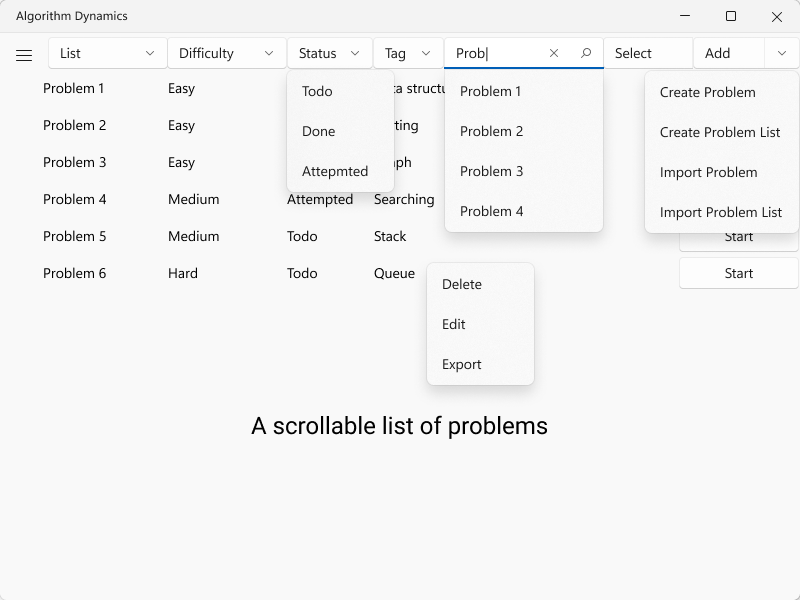
\includegraphics[width=\textwidth, height=\textheight, keepaspectratio]{ProblemsPage-Design}

The ProblemsPage displays problems in the database. The user can search, create, edit, delete, import, export or start working on one or multiple problems on this page.

\subsubsection{Usability Feature}

The user can apply selection condition by either select different fields in the dropdown boxes or directly type into the search box. A scrollable list of problems that match the conditions will be shown bellow, with detailed information. The user can start working on a problem by clicking the start button on the right. They can also right click the problem to call a context menu that includes more actions for them to delete, edit or export the problem. By clicking the select button on the top, the user can select multiple problems at once and applie the same action to them at once. By clicking the Add button on the top right, a context menu will be displayed, allowing the user to create or import new problems or problem lists. When the user is typing into the search box, a flyout will display matching results to save typing.

\subsubsection{Validation}

Most components on this page are still buttons, user can only click them and no invalid data can be input. The search box is where the user can input some text only, first, a flyout will be displayed to promote the user to click the button instead of inputting data themselves. Next, a length check will be applied, The user can only enter a maximum of 32 characters so they cannot crash the search box and the searching algorithm. Instead of passing the search keywords directly to the database, a custom searching algorithm will be used to search and sanitise the search keyword, which prevent SQL injection and provide a better searching experience.

\subsection{CodingPage}

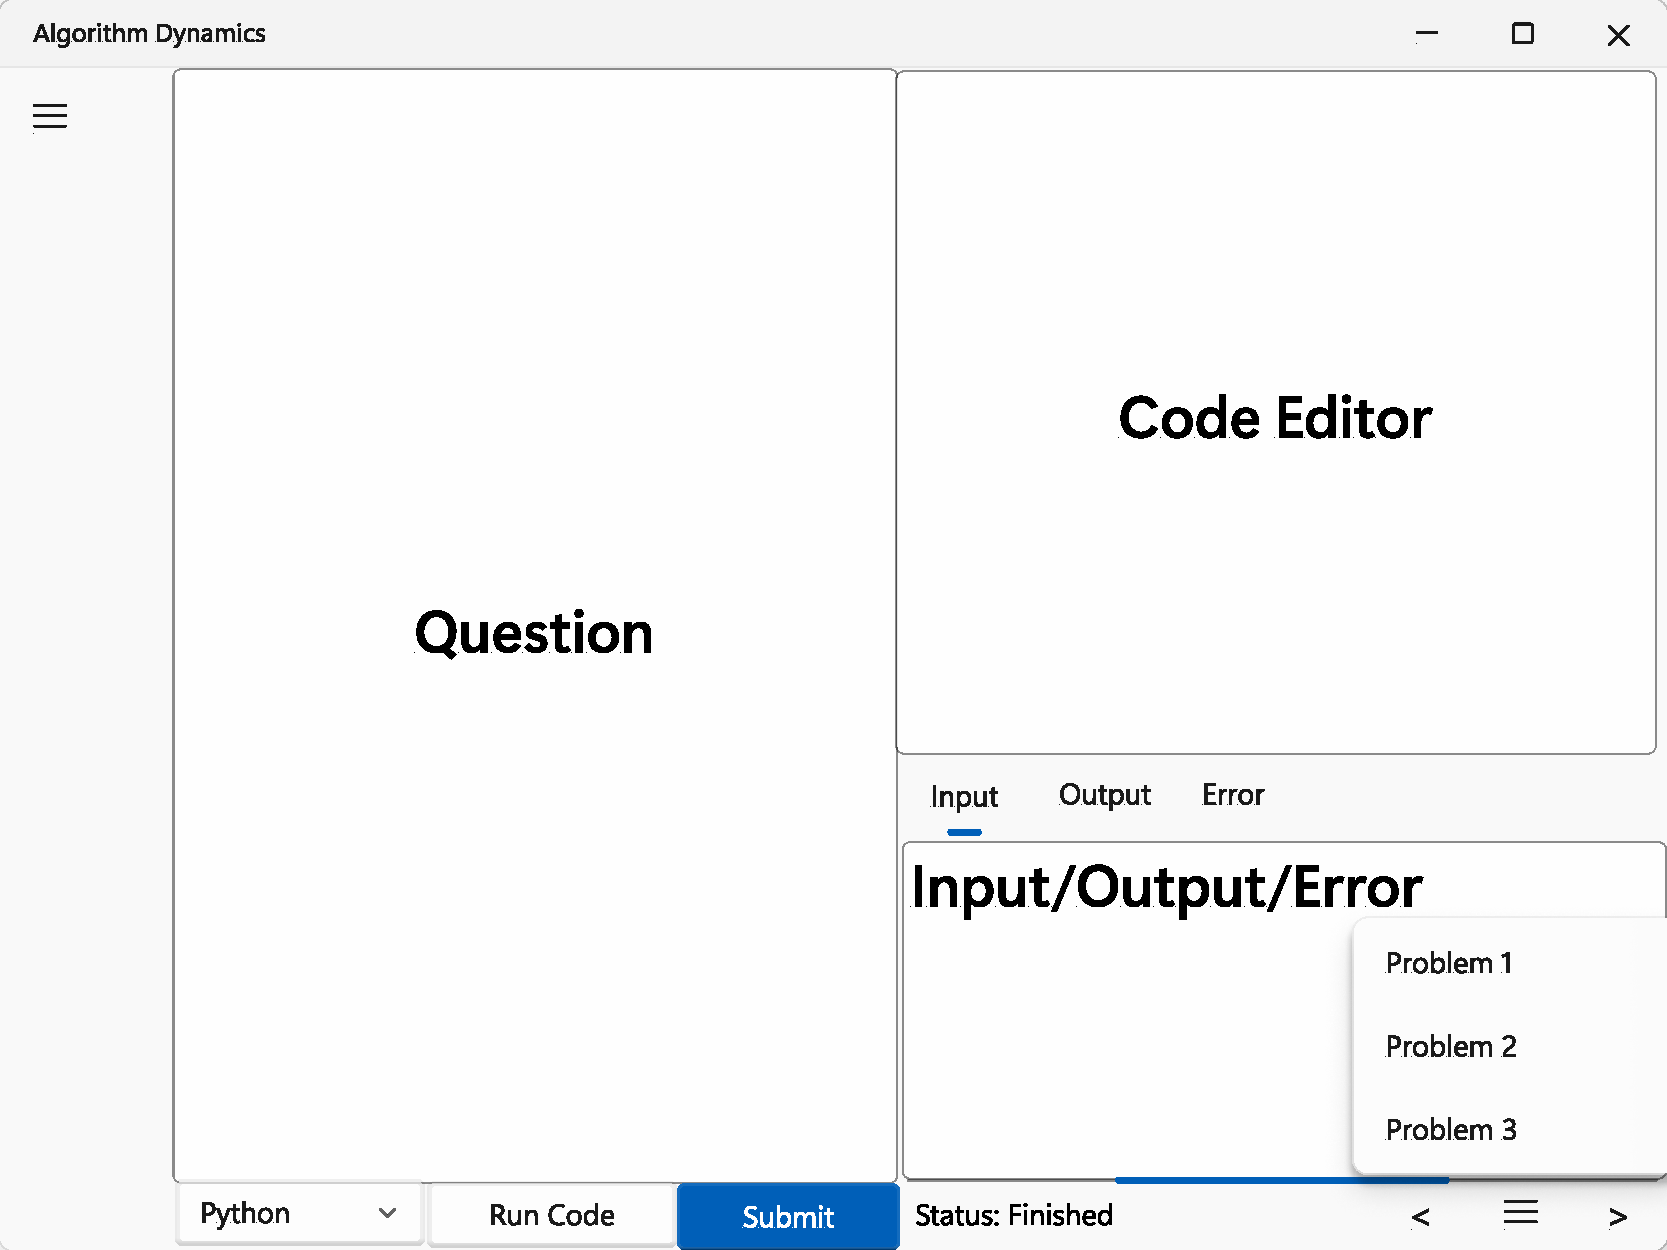
\includegraphics[width=\textwidth, height=\textheight, keepaspectratio]{CodingPage-Design}

The CodingPage is where the user works on a programming problem.

\subsubsection{Usability Feature}

The question is displayed on the left and a code editor will be displayed on the top right. The input, output and error messages will be displayed on button right, the user can switch between them by clicking the corresponding tab. On the button, the user can select programming language use a dropdown menu, run code by clicking the run code button and submit their code for judging by clicking the submit button. The status field shows the status of the judger and 3 navigation buttons on the button right to make it easy navigating between different problems. There is a progress bar between the input output error section and the navigation buttons, it displays the judging progress.  

\subsubsection{Validaton}

Again, most of the components on the page are either readonly (such as the question section) or buttons. The code editor is the only place for the user to input text, and the text inside will be validate by the compiler or ther intrepreter of the selected programming language. However, the input, output and error panel requires further validation. To prevent the user from printing out a huge amount of data which might results in poor performance, the input output error panel will perform a length check and only display the first 2048 characters of the output. 

\subsection{AssignmentsPage}

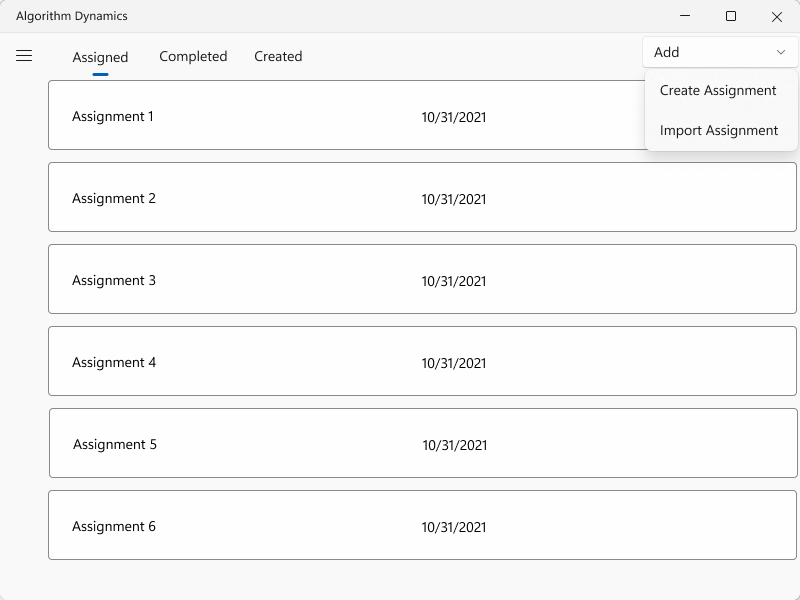
\includegraphics[width=\textwidth, height=\textheight, keepaspectratio]{AssignmentsPage-Design}

The AssignmentPage is where the user interact with their assignments. For student users, they can work on their assignments, for teacher users, they can create and mark assignments.

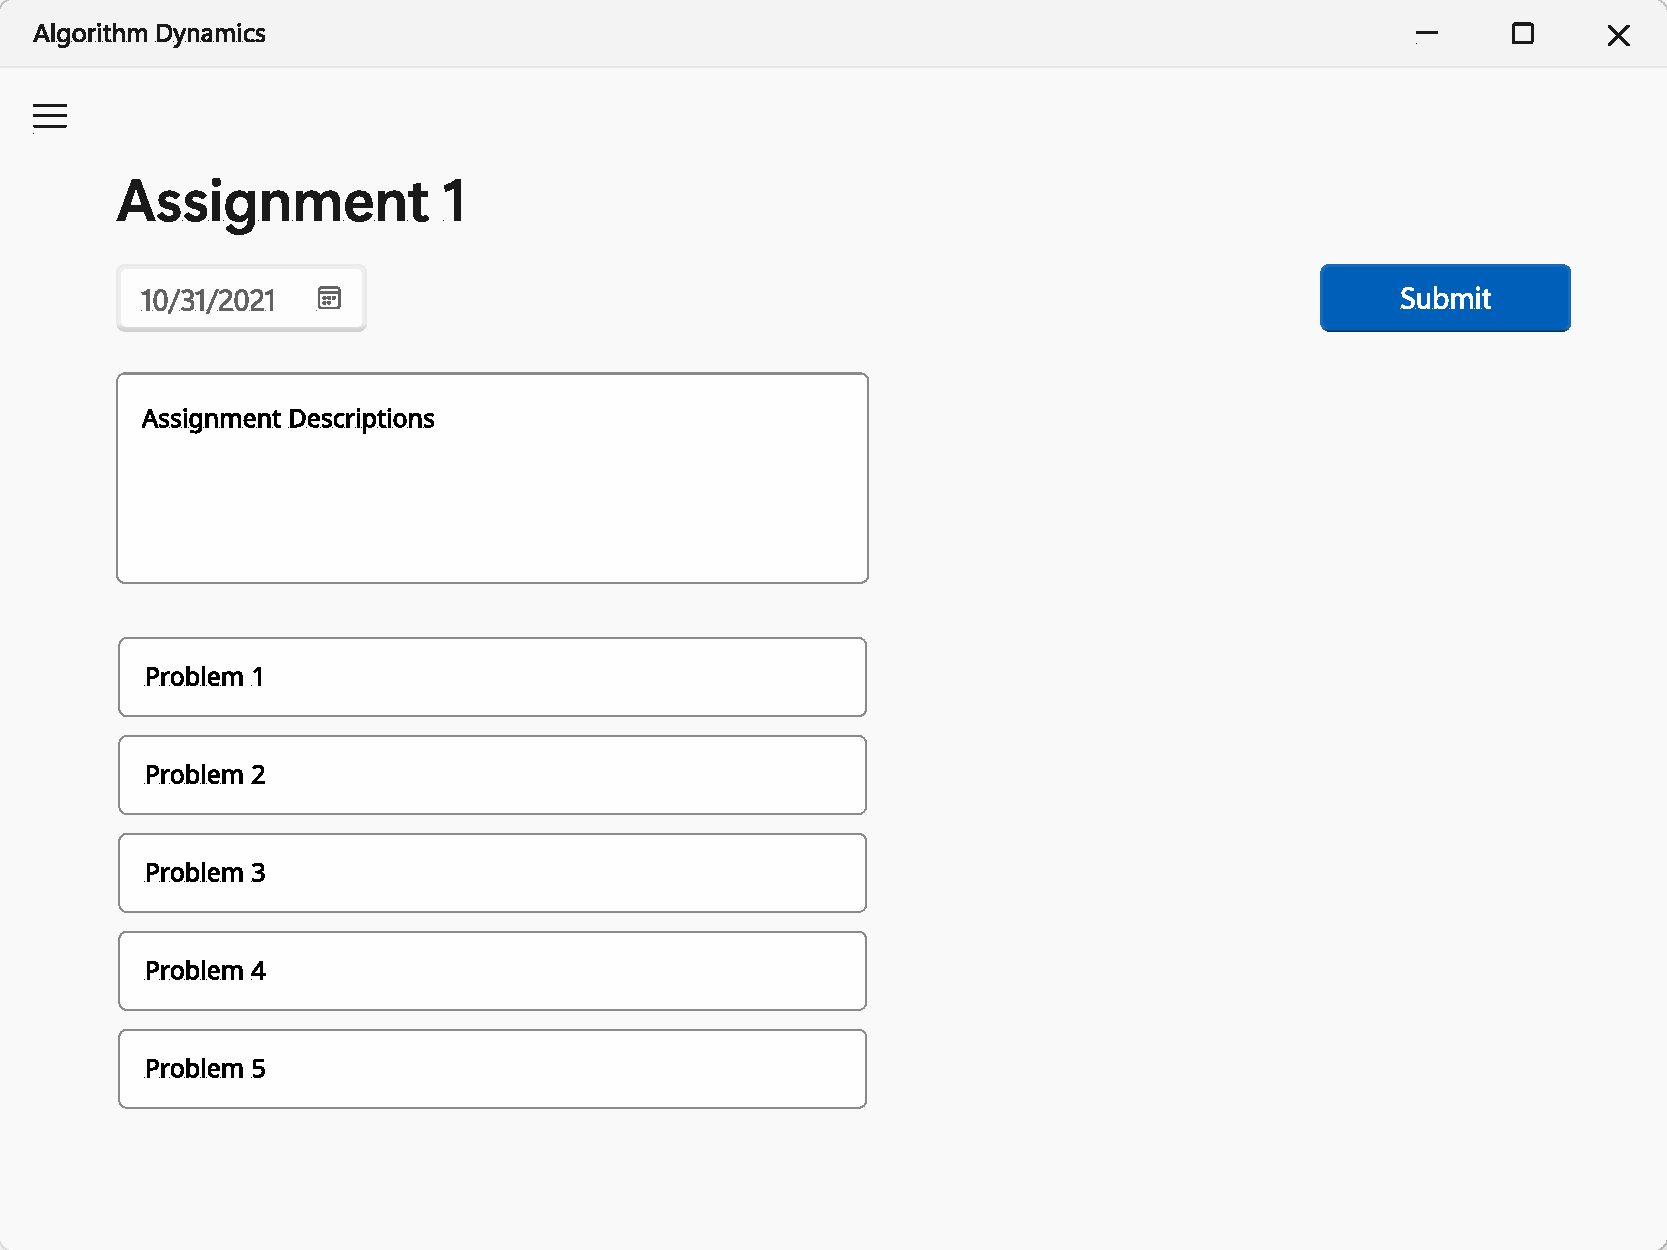
\includegraphics[width=\textwidth, height=\textheight, keepaspectratio]{AssignmentsStudentDetailsPage-Design}

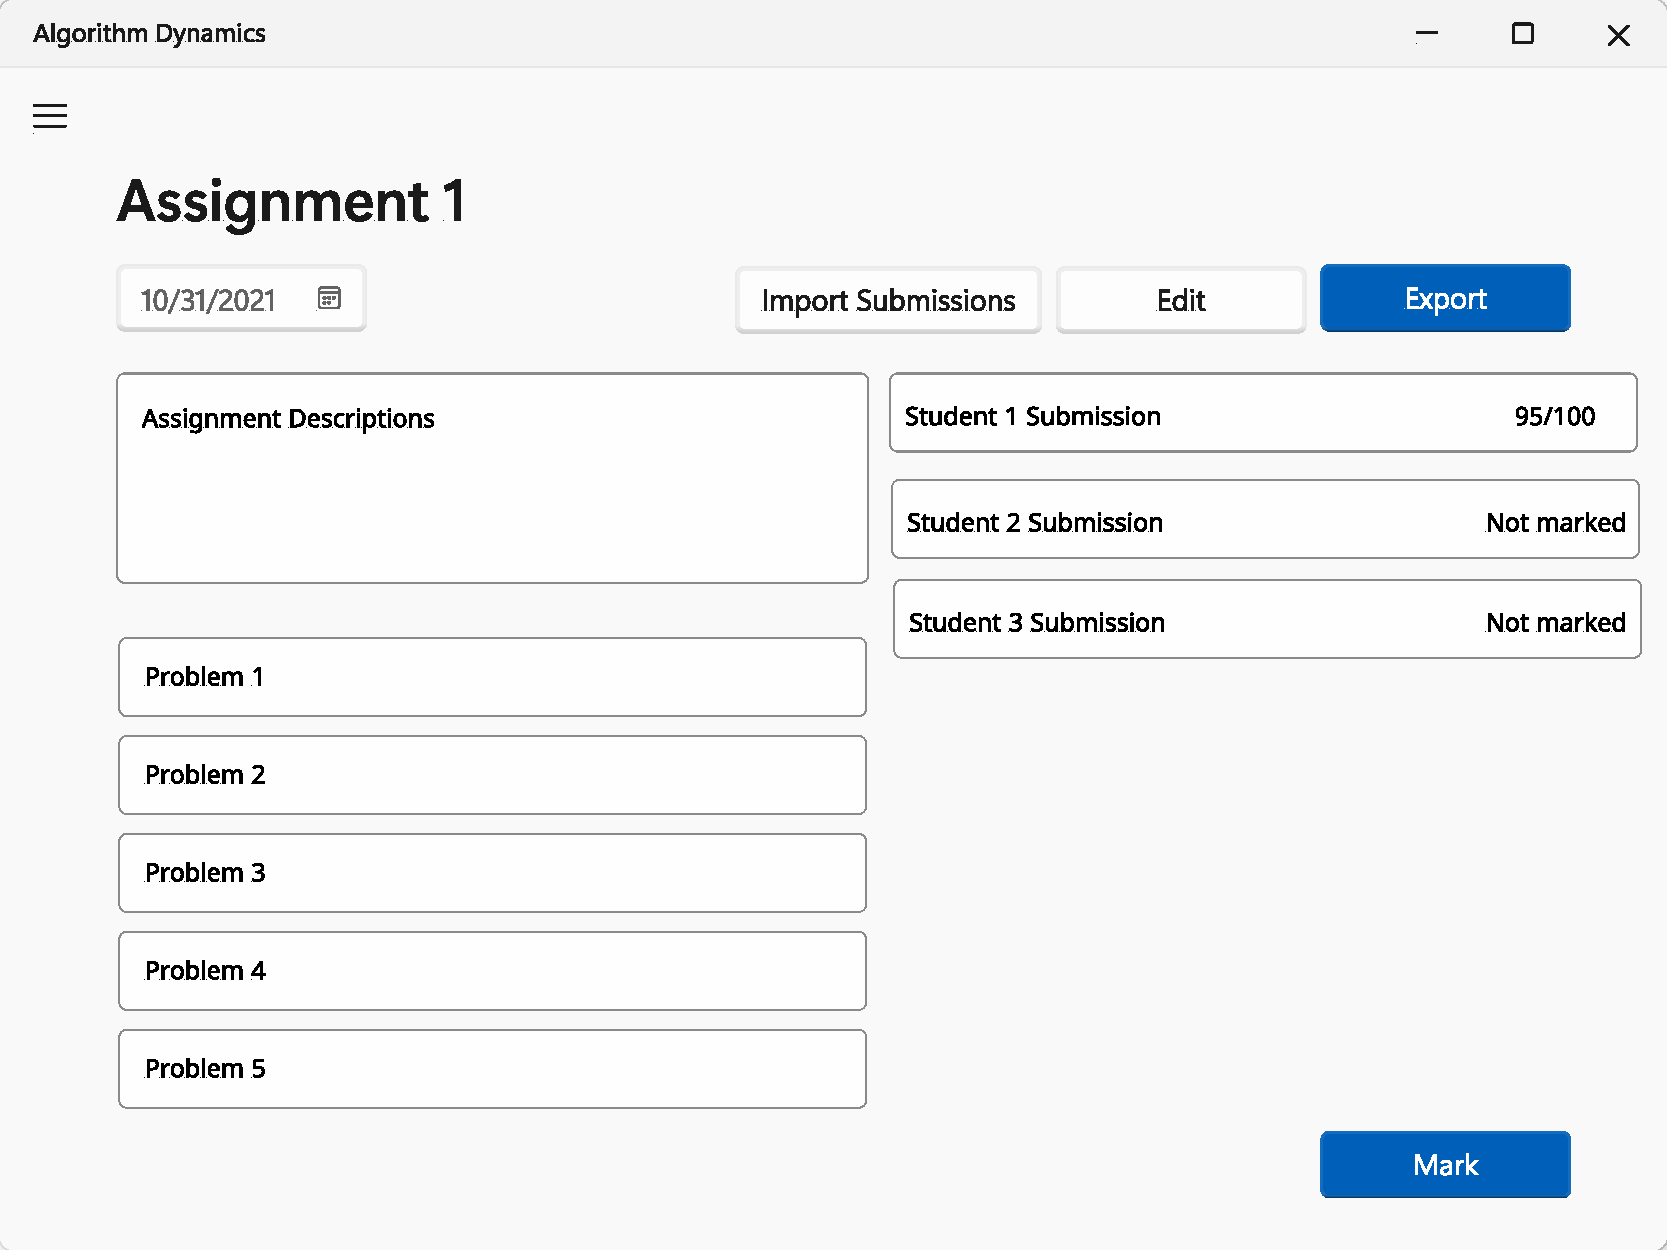
\includegraphics[width=\textwidth, height=\textheight, keepaspectratio]{AssignmentsTeacherDetailsPage-Design}

\subsection{PlaygroundPage}

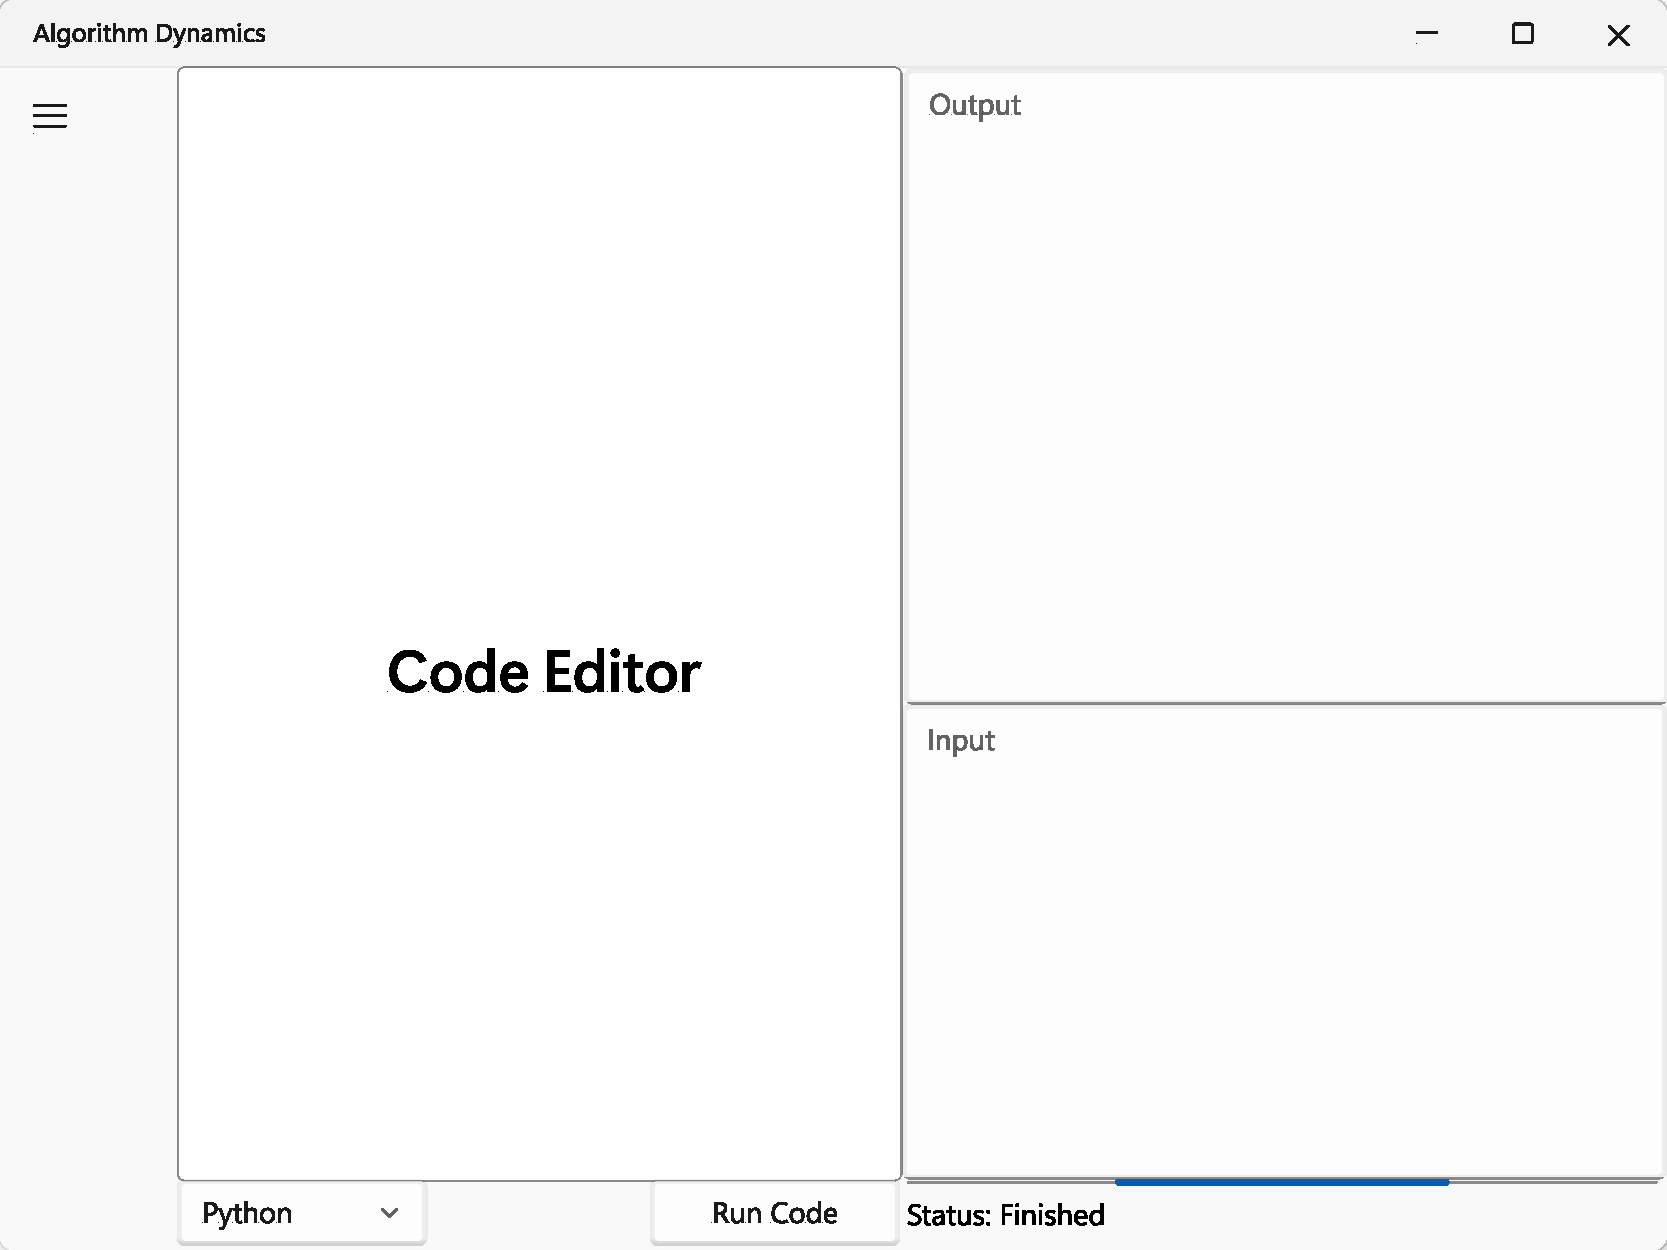
\includegraphics[width=\textwidth, height=\textheight, keepaspectratio]{PlaygroundPage-Design}

\subsection{AccountPage}

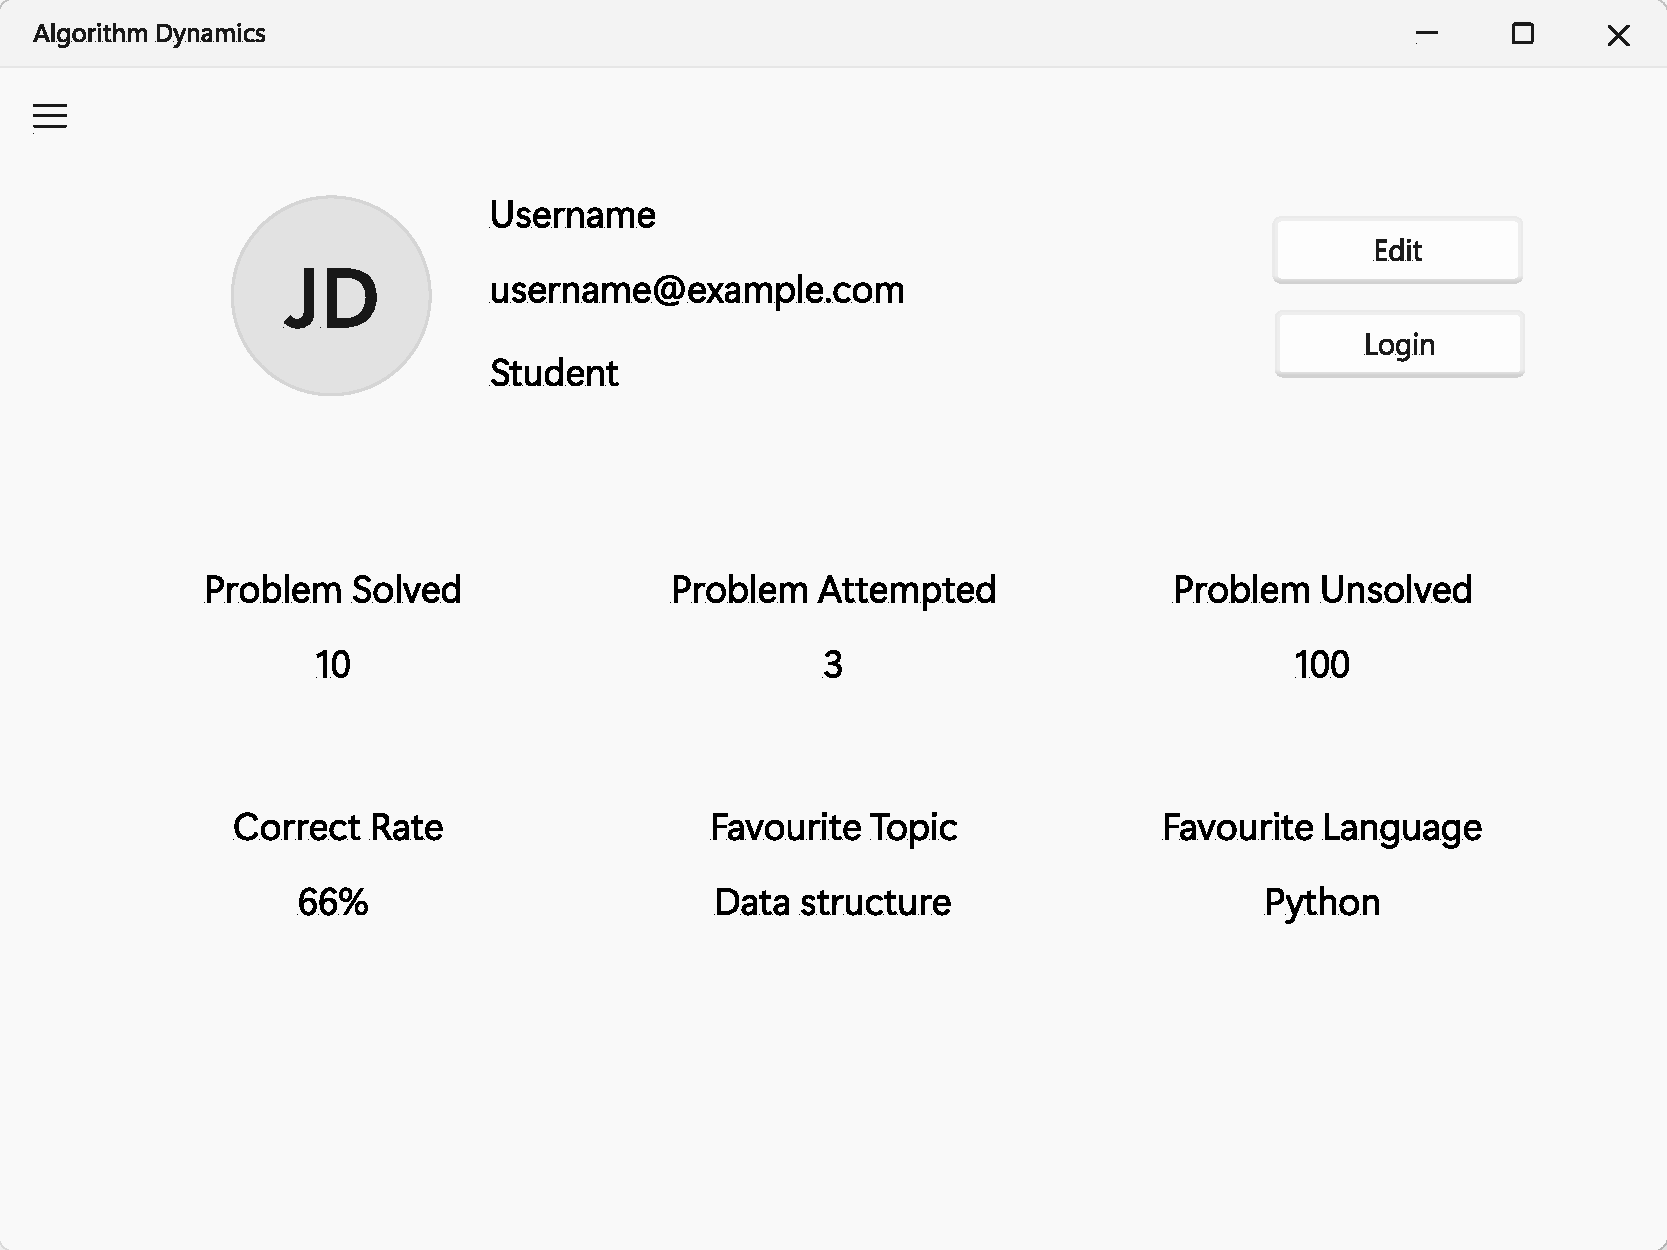
\includegraphics[width=\textwidth, height=\textheight, keepaspectratio]{AccountPage-Design}

\subsection{SettingsPage}

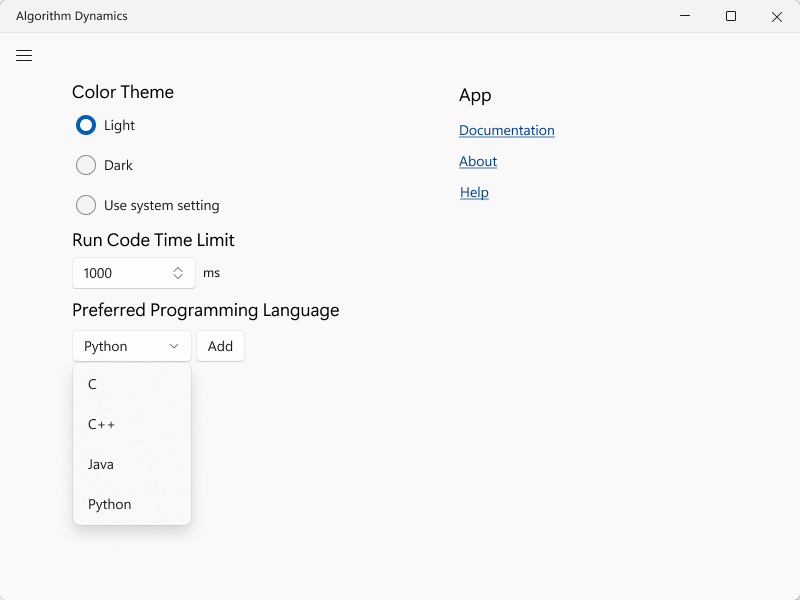
\includegraphics[width=\textwidth, height=\textheight, keepaspectratio]{SettingsPage-Design}

\subsection{CreateNewProblemPage}

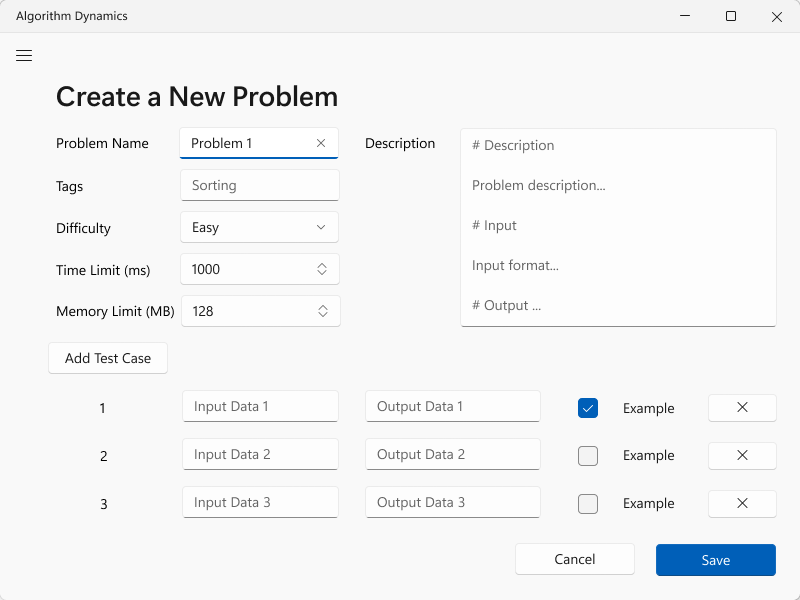
\includegraphics[width=\textwidth, height=\textheight, keepaspectratio]{CreateNewProblemPage-Design}

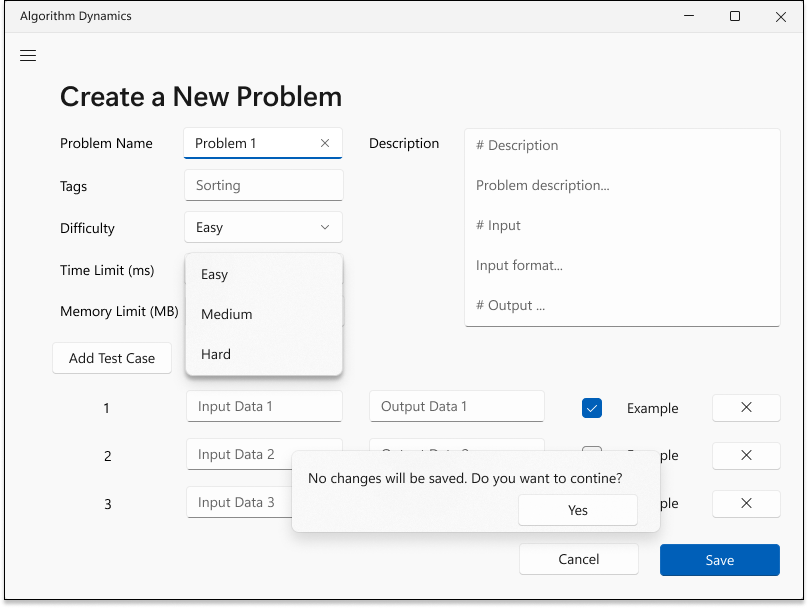
\includegraphics[width=\textwidth, height=\textheight, keepaspectratio]{CreateNewProblemPage-Expand-Design}

\subsection{CreateNewProblemListPage}

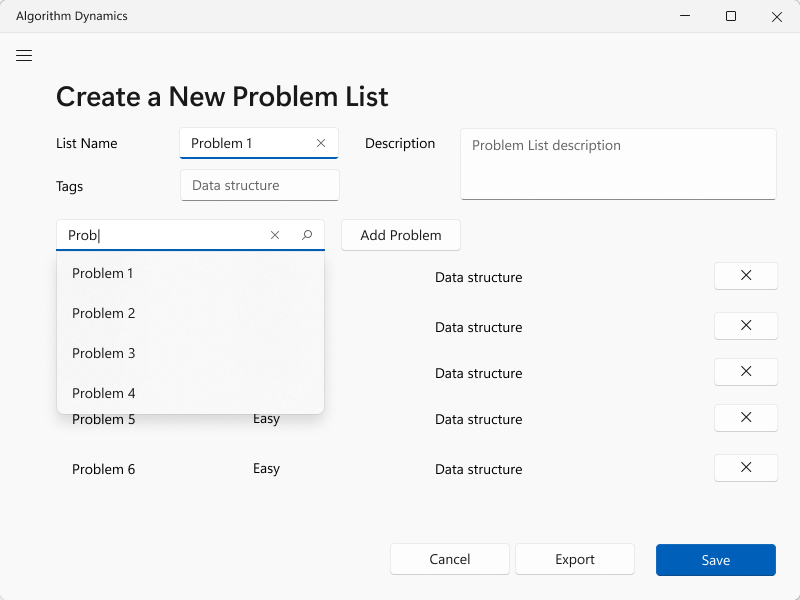
\includegraphics[width=\textwidth, height=\textheight, keepaspectratio]{CreateNewProblemListPage-Design}

\subsection{CreateNewAssignmentPage}

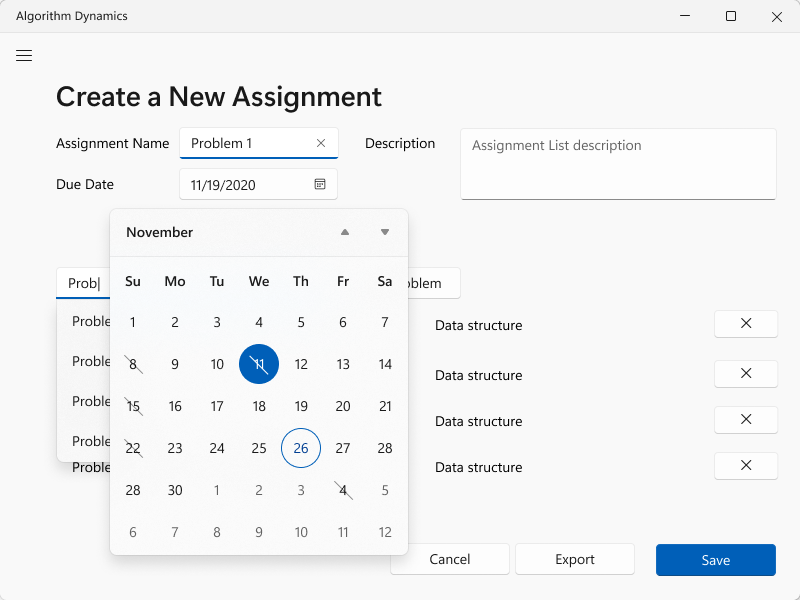
\includegraphics[width=\textwidth, height=\textheight, keepaspectratio]{CreateNewAssignmentPage-Design}

\subsection{Judger module}

\subsection{Database module}

Because this software will store many complex relational data, a relational database is needed to store all the data. Since the software runs locally, and every user will have different data, instead of a central SQL Server, a local SQL Database engine is required.

I choose to use SQLite to power this software. It is a small, self-contained, high-reliability, full-featured SQL Database engine, which will be enough to handle all the data storing and querying requests. Details about the desgin of the database will be described in the Data structure design section.

\subsection{REST API module}

\section{Algorithm design}

\subsection{Searchbox Searching Algorithm}

This algorithm will be used to power all the search boxes in the software. It will be packed into a function, taking in a list of item and the searching keyword input by the user, returning a list of results. To make the software easy to use, instead of simply using a linear search and returning all matching results, the algorithm will perform some fuzzy searching, so even the word is not typed in completely, matching results will be returned.

\begin{minted}[linenos,tabsize=4,breaklines]{text}
function search(List<string> sourceList, string keyword)
    // Create an empty list to store the results
    resultList = new List<string>()
    // Split the keyword into pieces by space
    splitKeyword = keyword.ToLower().Split(' ')
    // Compare each piece of keyword with the sourceList
    // Add the matching result into resultList
    for i=0 to sourceList.Length - 1
        for j=0 to splitKeyword.Length - 1
        sourceKey = sourceList[i].ToLower()
            if sourceKey.Contains(splitKeyword[j]) then
                resultList.Add(sourceList[i])
            endif
        next j
    next i

    // If no result is found,
    // add an "not found" notice to the resultList
    if resultList.Length == 0 then
          resultList.Add("No results found")
    endif
endfunction
\end{minted}

In this algorithm, I first create an empty list to store the result. Then I split the keyword into a list by space. So the keyword \mintinline{text}{"A Long Problem Name"} will be splitted into \mintinline{text}{["A", "Long", "Problem", "Name"]}.

Next, I use two nested loops to perform linear search on each splitted keyword. I choose to use linear search here because the list is not sorted, so only it will work. The overall time complexity here is $O(nm)$ where $n$ is the length of the \mintinline{text}{sourceList} and $m$ is the length of \mintinline{text}{splitKeyword}. This is not very fast, but in real word use cases, both $n$ and $m$ will be very small (less than 1000), so this algorithm will be fast enough to handle most of the cases. The increase in complexity brings a better searching experience. In this way, the algorithm will be able to match keywords like \mintinline{text}{prob} to result \mintinline{text}{A Long Problem List}, while normal linear search will not be able to do this.

At the end, if no item is found, a not found notice is added to the list, which will be displayed to the user.

\subsection{Judger RunCode Algorithm}

This algorithm is designed for the \mintinline{text}{Judger} to run a piece of code, pass input to the code and receive all the output and error. This is the basic function of the \mintinline{text}{Judger} and further judging will all based on this algorithm. An async function will be used so it will not block the main UI thread. It takes three input, \mintinline{text}{UserCode} for the code to be executed, \mintinline{text}{Input} for the input data, and TODO for the programming language. There are two types of programming languages, interpreted programming languages and complied programming languages, the procedure to run them is quite different, so I need to handle them separately. The configuration for each language is stored as \mintinline{text}{LanguageConfig}.


\begin{minted}[linenos,tabsize=4,breaklines]{text}
async function RunCode(string UserCode, string Input, Language language)


endfunction
\end{minted}

\subsection{Judger Judge Problem Algorithm}

\subsection{Judger Judge Assignment Algorithm}

\section{Data structure design}

\subsection{Class design}

I am taking an object-oriented approach to the design of the software. This is the class diagram for all classes.

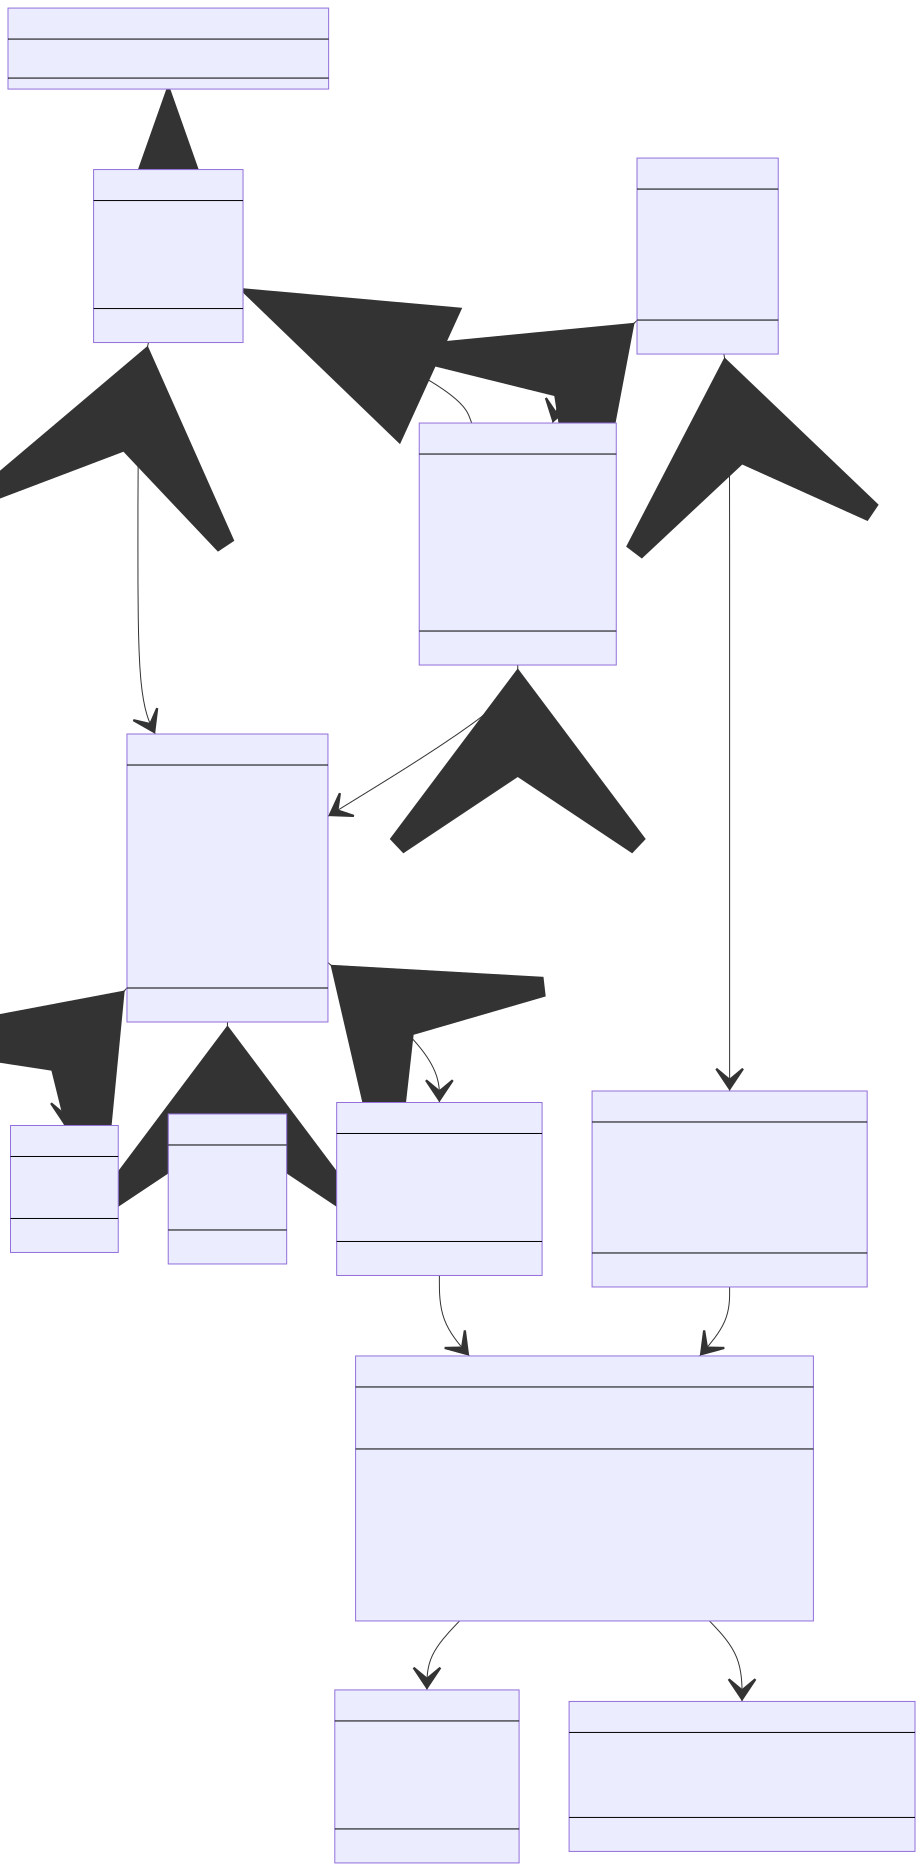
\includegraphics[width=\textwidth, height=\textheight, keepaspectratio]{classDiagram}

\subsubsection{\mintinline{text}{User}}

The \mintinline{text}{User} object is used to manage the current user. Its data will be recorded attached to \mintinline{text}{Submission}, \mintinline{text}{Assignment} and \mintinline{text}{AssignmentSubmission}.

\begin{tabulary}{\textwidth}{|l|l|L|}
    \hline
    Variable & Data type & Justification \\
    \mintinline{text}{Uid} & \mintinline{text}{Guid} & global unique identifier \\
    \hline
    \mintinline{text}{FirstName} & \mintinline{text}{string} & first name of the user \\
    \hline
    \mintinline{text}{LastName} & \mintinline{text}{string} & last name of the user \\
    \hline
    \mintinline{text}{Email} & \mintinline{text}{string} & Email address of the user \\
    \hline
    \mintinline{text}{Role} & \mintinline{text}{enum Role} & Whether the user is a teacher or a student. \\
    \hline
\end{tabulary}

\subsubsection{\mintinline{text}{Tag}}

A \mintinline{text}{Tag} is a label used to categorize a \mintinline{text}{Problem}.

\begin{tabulary}{\textwidth}{|l|l|L|}
    \hline
    Variable & Data type & Justification \\
    \hline
    \mintinline{text}{Id} & \mintinline{text}{int} & The \mintinline{text}{Id} is the local unique identifier for a \mintinline{text}{Tag}, it comes in handy when I need to store a \mintinline{text}{Tag} into the database. \\
    \hline
    \mintinline{text}{Name} & \mintinline{text}{string} & The \mintinline{text}{Name} of the \mintinline{text}{Tag} specifics the content of the \mintinline{text}{Tag}. I use \mintinline{text}{string} as the data type so a string of characters can be stored for its name. \\
    \hline
\end{tabulary}

\subsubsection{\mintinline{text}{TestCase}}

A \mintinline{text}{TestCase} is one set of test input and output, which will be used by the \mintinline{text}{Judger} to judge user's submission.

\begin{tabulary}{\textwidth}{|l|l|L|}
    \hline
    Variable & Data type & Justification \\
    \hline
    \mintinline{text}{Id} & \mintinline{text}{int} & The \mintinline{text}{Id} is the local unique identifier for a \mintinline{text}{TestCase}, it comes in handy when I need to store a \mintinline{text}{TestCase} into the database. \\
    \hline
    \mintinline{text}{Input} & \mintinline{text}{string} & The \mintinline{text}{Input} will be feed to the user's submission code by the \mintinline{text}{Judger}. \\
    \hline
    \mintinline{text}{Output} & \mintinline{text}{string} & This stores the expected \mintinline{text}{Output} of the \mintinline{text}{Input}. The \mintinline{text}{Judger} will compare user's output with the \mintinline{text}{Output} to judge whether user's code is correct. \\
    \hline
    \mintinline{text}{IsExample} & \mintinline{text}{bool} & Define whether this \mintinline{text}{TestCase} is an example. An example \mintinline{text}{TestCase} will be displayed to the user for debugging, and distribute with an \mintinline{text}{Assignment}. A non-example \mintinline{text}{TestCase} will be used to judge the solution and will not be displayed to the user or distribute with an \mintinline{text}{Assignment}. A boolean value is suitable to store the two-state data. \\
    \hline
\end{tabulary}

\subsubsection{\mintinline{text}{Problem}}

The \mintinline{text}{Problem} is the core data object of this program. It is used to store and organize the data for each individual programming question.

\begin{tabulary}{\textwidth}{|l|l|L|}
    \hline
    Variable & Data type & Justification \\
    \hline
    \mintinline{text}{Id} & \mintinline{text}{int} & The \mintinline{text}{Id} is the local unique identifier for a \mintinline{text}{Problem}, it comes in handy when I need to store a \mintinline{text}{Problem} into the database. When exporting a \mintinline{text}{Problem}, the \mintinline{text}{Id} will not be exported. Instead, a new \mintinline{text}{Id} is given when the other user imports the \mintinline{text}{Problem}. \\
    \hline
    \mintinline{text}{Name} & \mintinline{text}{string} & The \mintinline{text}{Name} is a string contains the name of a \mintinline{text}{Problem}. \\
    \hline
    \mintinline{text}{Description} & \mintinline{text}{string} & The \mintinline{text}{Description} is a string storing the detailed description of a \mintinline{text}{Problem}. Markdown syntax is supported for a better user experience. \\
    \hline
    \mintinline{text}{Status} & \mintinline{text}{enum Status} & \mintinline{text}{Status} is an enumeration type containing 3 possible status: \mintinline{text}{Todo}, \mintinline{text}{Solved} and \mintinline{text}{Attempted}. This is used to collect user statistics data. I choose to use a custom enumeration type instead of some magic numbers to make the code more readable and easier to maintain. \\
    \hline
    \mintinline{text}{Difficulty} & \mintinline{text}{enum Difficulty} & \mintinline{text}{Difficulty} is an enumeration type containing 3 possible difficulties: \mintinline{text}{Easy}, \mintinline{text}{Medium} and \mintinline{text}{Hard}. This provdes a way for the user to search and select problems by their difficulties. \\
    \hline
    \mintinline{text}{TimeLimit} & \mintinline{text}{int} & \mintinline{text}{TimeLimit} sets the max time allowed for the user code to run in millisecond. When the running time exceed the \mintinline{text}{TimeLimit}, the running code will be killed and a Time Limit Exceed error will be recorded. This prevents infinite loop from using up all computing resources and rejects inefficient algorithms. \\
    \hline
    \mintinline{text}{MemoryLimit} & \mintinline{text}{int} & \mintinline{text}{MemoryLimit} sets the max memory allowed for the user's code to consume in bytes. When the memory usage exceed the memory limit, the running code will be killed and a Memory Limit Exceed Error will be recorded. This prevents incorrect code from using up all memory space and rejects inefficient algorithms. \\
    \hline
\end{tabulary}

\begin{tabulary}{\textwidth}{|l|l|L|}
    \hline
    Variable & Data type & Justification \\
    \hline
    \mintinline{text}{TestCases} & \mintinline{text}{List<TestCase>} & \mintinline{text}{TestCases} is a list containing all \mintinline{text}{TestCase} for the problem. A list is more appropriate than an array because it allows new \mintinline{text}{TestCase} to be added or remove existing ones during runtime. \\
    \hline
    \mintinline{text}{Tags} & \mintinline{text}{List<Tags>} & \mintinline{text}{Tags} is a list containing all \mintinline{text}{Tags} for a \mintinline{text}{Problem}. Similarly, I use a list for \mintinline{text}{Tags} so it can be added or removed during runtime. \\
    \hline
\end{tabulary}

\subsubsection{\mintinline{text}{Language}}

The \mintinline{text}{Language} class defines the compiling and running configurations for different programming languages. This part is hard coded into the code and will not expose to the user as explained in the Limitation setion. Thus, it does not require an \mintinline{text}{Id} attribute since it will not be stored in the database.

\begin{tabulary}{\textwidth}{|l|l|L|}
    \hline
    Variable & Data type & Justification \\
    \hline
    \mintinline{text}{Name} & \mintinline{text}{string} & I use a \mintinline{text}{string} variable to store the \mintinline{text}{Name} of a programming language. This \mintinline{text}{Name} will be displayed in the drop down menu for the user to select preferred programming language. \\
    \hline
    \mintinline{text}{NeedCompile} & \mintinline{text}{bool} & Some programming languages need to be compiled before running, such as C, C++ and Java. This attribute is used to tell the \mintinline{text}{Judger} to compile before executing. \\
    \hline
    \mintinline{text}{CompileCommand} & \mintinline{text}{string} & If a programming language requires compilation, this command is executed to call the compiler. \\
    \hline
    \mintinline{text}{CompileArguments} & \mintinline{text}{string} & If a programming language requires compilation, this arguments is passed to the command, to specify related file path and compile arguments. \\
    \hline
    \mintinline{text}{RunCommand} & \mintinline{text}{string} & The \mintinline{text}{Judger} uses this command to run the executable or the intrepreter. \\
    \hline
    \mintinline{text}{RunArguments} & \mintinline{text}{string} & This \mintinline{text}{Judger} pass this arguments to the executable or the intrepreter. \\
    \hline
\end{tabulary}

\subsubsection{\mintinline{text}{Submission}}

A \mintinline{text}{Submission} is created when the user submits a code solution to the \mintinline{text}{Judger}. The \mintinline{text}{Submission} will contain all the information including the time, the source code, the programming language selected and the corresponding \mintinline{text}{Problem} for the \mintinline{text}{Judger} to judge.

\begin{tabulary}{\textwidth}{|l|l|L|}
    \hline
    Variable & Data type & Justification \\
    \hline
    \mintinline{text}{Id} & \mintinline{text}{int} & This \mintinline{text}{Id} is the local unique identifier for a \mintinline{text}{Submission}, it comes in handy when I need to store a \mintinline{text}{Submission} into the database. \\
    \hline
    \mintinline{text}{Problem} & \mintinline{text}{Problem} & The \mintinline{text}{Problem} contains the corresponding \mintinline{text}{Problem} of this \mintinline{text}{Submission}, which also contains the \mintinline{text}{TestCases} for the \mintinline{text}{Judger} to judge the \mintinline{text}{Submission}. Before storing a \mintinline{text}{Submission} into the database, this value needs to be normalized to the \mintinline{text}{Id} of that \mintinline{text}{Problem}. \\
    \hline
    \mintinline{text}{Code} & \mintinline{text}{string} & \mintinline{text}{Code} stores the submitted code, which will be executed and judged by the \mintinline{text}{Judger}. \\
    \hline
    \mintinline{text}{SubmittedTime} & \mintinline{text}{DateTime} & \mintinline{text}{SubmittedTime} stores the time the \mintinline{text}{Submission} is created. Instead of using a \mintinline{text}{string} or an \mintinline{text}{int} value, I decide to use the native data type \mintinline{text}{DateTime} provided by C\#, which makes it easier to process date time, and prevent any formating issues. \\
    \hline
    \mintinline{text}{Language} & \mintinline{text}{enum Language} & \mintinline{text}{Language} stores the programming language selected by the user, so the \mintinline{text}{Judger} knows how to run the code.\\
    \hline
\end{tabulary}

\subsubsection{\mintinline{text}{ProblemList}}

A \mintinline{text}{ProblemList} is a list of \mintinline{text}{Problem}, with a list of \mintinline{text}{Tags} so the user can share a list of problems easily. It is also the parent of \mintinline{text}{Assignment} and provides basic functions for it. The \mintinline{text}{ProblemList} is inheriate from the \mintinline{text}{List<Problem>} class, which is provded by the .NET 5 library. \mintinline{text}{List<Problem>} provides all basic functions for a list, such as add, remove, sort and find, so I don't need to reinvent the wheel. I choose a list instead of an array because the number of \mintinline{text}{Problem} inside the list will be changed during runtime, so a list is more appropriate for my use case.

\begin{tabulary}{\textwidth}{|l|l|L|}
    \hline
    Variable & Data type & Justification \\
    \hline
    \mintinline{text}{Id} & \mintinline{text}{int} & This \mintinline{text}{Id} is the local unique identifier for a \mintinline{text}{ProblemList}, it comes in handy when I need to store a \mintinline{text}{ProblemList} into the database. \\
    \hline
    \mintinline{text}{Name} & \mintinline{text}{string} & The name is a string to store the name of the problem list. \\
    \hline
    \mintinline{text}{Description} & \mintinline{text}{string} & The description is a string to store the description of a \mintinline{text}{ProblemList}. \\
    \hline
\end{tabulary}

\subsubsection{\mintinline{text}{Assignment}}

An \mintinline{text}{Assignment} is a \mintinline{text}{ProblemList} with descriptions and a due date. Because the assignment needs to be distributed to students, it is a little more complicated. When an \mintinline{text}{Assignment} is distributed, a copy of that \mintinline{text}{Assignment} is created. All \mintinline{text}{TestCases} with \mintinline{text}{IsExample} set to \mintinline{text}{false} will be removed to prevent students from cheating. The \mintinline{text}{Type} of the \mintinline{text}{Assignment} will be set to \mintinline{text}{Copy} to indicate it is a distributed copy. The \mintinline{text}{Judger} will reject to judge a distributed \mintinline{text}{Assignment} and the \mintinline{text}{AssignmentsPage} will show the \mintinline{text}{Assignment} under the Assigned tab instead of the Created tab.

\mintinline{text}{Assignment} is inheriate from the \mintinline{text}{ProblemList}, so it can reuse the \mintinline{text}{Name} and \mintinline{text}{Description} attributes and all methods  to manage a list of \mintinline{text}{Problem}. Upon that, new attributes and methods are added to make it functional.

\begin{tabulary}{\textwidth}{|l|l|L|}
    \hline
    Variable & Data type & Justification \\
    \hline
    \mintinline{text}{Uid} & \mintinline{text}{Guid} & The \mintinline{text}{Assignment} will use a \mintinline{text}{Guid} value for its \mintinline{text}{Uid} instead of a normal \mintinline{text}{int} value to ensure the \mintinline{text}{Uid} is unique globally. So when the user import an \mintinline{text}{Assignment} into their database, the \mintinline{text}{Uid} will not conflict with any existing values, and it will not be changed (Unlike a \mintinline{text}{ProblemList}, for which will be assigned a new \mintinline{text}{Id} when importing). The \mintinline{text}{Uid} will be referenced by the \mintinline{text}{AssignmentSubmission} so the \mintinline{text}{Judger} will be able to know which \mintinline{text}{Assignment} it is judging. \\
    \hline
    \mintinline{text}{DueDate} & \mintinline{text}{DateTime} & The \mintinline{text}{DueDate} stores the time for the due date of the \mintinline{text}{Assignment}. Instead of using a \mintinline{text}{string} or an \mintinline{text}{int} value, I decide to use the native data type \mintinline{text}{DateTime} provided by C\#, which makes it easier to process date time, and prevent all formating issues. \\
    \hline
    \mintinline{text}{Status} & \mintinline{text}{enum Status} & \mintinline{text}{Status} is an enumeration type containing 4 possible status for a source \mintinline{text}{Assignment}: \mintinline{text}{Draft}, \mintinline{text}{Scheduled}, \mintinline{text}{Published} and \mintinline{text}{Assigned} for the teacher to manage the lifecycle of an \mintinline{text}{Assignment}. For a distributed \mintinline{text}{Assignment}, there are 4 possible \mintinline{text}{Status}, \mintinline{text}{NotStarted}, \mintinline{text}{InProgress}, \mintinline{text}{Completed} and \mintinline{text}{OverDue}, which helps the student to manage the lifecycle of an \mintinline{text}{Assignment}. I choose to use a custom enumeration type instead of some magic numbers to make the code more readable and easier to maintain.\\
    \hline
    \mintinline{text}{Type} & \mintinline{text}{enum Type} & \mintinline{text}{Type} is an enumeration type containing 2 possible types, \mintinline{text}{Source} or \mintinline{text}{Copy}. It is used to manage the distribution of an \mintinline{text}{Assignment} as described above. \\
    \hline
\end{tabulary}

When a student finishes an \mintinline{text}{Assignment}, an \mintinline{text}{AssignmentSubmission} is created for the \mintinline{text}{Judger} to judge. The \mintinline{text}{AssignmentSubmission} can either be exported to file and sent to the teacher, or it is uploaded using API. The teacher imports the \mintinline{text}{AssignmentSubmission} or uses API to load it, and the \mintinline{text}{Judger} will be able to mark it and give the result.

\subsubsection{\mintinline{text}{AssignmentSubmission}}

\begin{tabulary}{\textwidth}{|l|l|L|}
    \hline
    Variable & Data type & Justification \\
    \hline
    \mintinline{text}{Uid} & \mintinline{text}{Guid} & The \mintinline{text}{AssignmentSubmission} uses a \mintinline{text}{Guid} value for its \mintinline{text}{Uid} instead of a normal \mintinline{text}{int} value to ensure the \mintinline{text}{Uid} is unique globally. So when teachers import an \mintinline{text}{AssignmentSubmission} into their database, the \mintinline{text}{Uid} will not conflict with any existing values, and it will not be changed. \\
    \hline
    \mintinline{text}{Submitter} & \mintinline{text}{User} & The user information is collected when exporting an \mintinline{text}{AssignmentSubmission}, so the teacher will be able to know who is the \mintinline{text}{Submitter}. \\
    \hline
    \mintinline{text}{Assignment} & \mintinline{text}{Assignment} & The \mintinline{text}{Assignment} corresponding to this \mintinline{text}{AssignmentSubmission}, so the \mintinline{text}{Judger} knows how to judge it. \\
    \hline
    \mintinline{text}{Status} & \mintinline{text}{enum Status} & \mintinline{text}{Status} is an enumeration type containing 3 possible types, \mintinline{text}{Source} or \mintinline{text}{Copy}. It is used to manage the distribution of an \mintinline{text}{Assignment} as described above. \\
    \hline
\end{tabulary}

\subsubsection{\mintinline{text}{Judger}}

The \mintinline{text}{Judger} is a static class, only eposes 4 functions to run and judge user's code. No variable is exposed and no data will be saved to the database. The private variables are discussed in the previous Algorithm design section.

\subsubsection{\mintinline{text}{TestCaseResult}}

The judging result for each individual \mintinline{text}{TestCase}.

\begin{tabulary}{\textwidth}{|l|l|L|}
    \hline
    Variable & Data type & Justification \\
    \hline
\end{tabulary}

\subsubsection{\mintinline{text}{SubmissionResult}}

When the \mintinline{text}{Judger} finishes judging a \mintinline{text}{Submission}, a \mintinline{text}{SubmissionResult} is created and stored. It includes the result and statistics about the \mintinline{text}{Submission}.

\begin{tabulary}{\textwidth}{|l|l|L|}
    \hline
    Variable & Data type & Justification \\
    \hline
    \mintinline{text}{Id} & \mintinline{text}{int} & This \mintinline{text}{Id} is the local unique identifier for a \mintinline{text}{SubmissionResult}, it comes in handy when I need to store a \mintinline{text}{SubmissionResult} into the database.\\
    \hline
    \mintinline{text}{Submission} & \mintinline{text}{Submission} & store the corresponding submission \\
    \hline
    \mintinline{text}{StandardOutput} & \mintinline{text}{string} & qwq \\
    \hline
    \mintinline{text}{StandardError} & \mintinline{}{}
    \hline
\end{tabulary}

\subsubsection{\mintinline{text}{AssignmentSubmissionResult}}

\begin{tabulary}{\textwidth}{|l|l|L|}
    \hline
    Variable & Data type & Justification \\
    \hline
\end{tabulary}

\subsection{Settings design}

The settings will be stored in a JSON file.

\begin{minted}[linenos,tabsize=4,breaklines]{json}
{
    "AppBackgroundRequestedTheme": "Light/Dark/System",
}
\end{minted}

\subsection{Database design}

\subsubsection{Tag Table}

\begin{tabulary}{\textwidth}{|L|L|}
    \hline
    Id & Name \\
    \hline
    1 & Tag1 \\
    \hline
\end{tabulary}

\begin{minted}[linenos,tabsize=4,breaklines]{sql}
CREATE TABLE Tag
(
    PRIMARY KEY(Id) INTEGER NOT NULL AUTO_INCREMENT,
    Name TEXT NOT NULL
)
\end{minted}

\subsubsection{ProblemTag Table}

The \mintinline{text}{Tag} has a many-to-many relation with the \mintinline{text}{Problem}. A \mintinline{text}{Problem} can have multiple \mintinline{text}{Tags} and a \mintinline{text}{Tag} can be assigned to multiple \mintinline{text}{Problems}. So a link table is required to normalize the data.

\begin{tabulary}{\textwidth}{|L|L|L|}
    \hline
    Id & ProblemId & TagId \\
    \hline
    1 & 1 & 1 \\
    \hline
    2 & 1 & 2 \\
    \hline
\end{tabulary}

\begin{minted}[linenos,tabsize=4,breaklines]{sql}
CREATE TABLE ProblemTag
(
    PRIMARY KEY(Id) INTEGER NOT NULL AUTO_INCREMENT,
    FOREIGN KEY (ProblemId) REFERENCES Problem(Id),
    FOREIGN KEY (TagId) REFERENCES Tag(Id),
)
\end{minted}

\subsubsection{TestCase Table}

The \mintinline{text}{TestCase} has a many-to-one relation to the \mintinline{text}{Problem}, one \mintinline{text}{Problem} can have multiple \mintinline{text}{TestCase} while one \mintinline{text}{TestCase} can only belong to one \mintinline{text}{Problem}. So, a foreign key \mintinline{text}{ProblemId} is enabled for the \mintinline{text}{TestCase} to store its corresponding \mintinline{text}{Problem}.

\begin{tabulary}{\textwidth}{|L|L|L|L|L|}
    \hline
    Id & Input & Output & IsExample & ProblemId \\
    \hline
    1 & ``Input1'' & ``Output1'' & true & 1 \\
    \hline
\end{tabulary}

\begin{minted}[linenos,tabsize=4,breaklines]{sql}
CREATE TABLE TestCase
(
    PRIMARY KEY(Id) INTEGER NOT NULL AUTO_INCREMENT,
    Input TEXT NOT NULL,
    Output TEXT NOT NULL,
    IsExample INTEGER NOT NULL,
    FOREIGN KEY (ProblemId) REFERENCES Problem(Id)
)
\end{minted}

\subsection{Input Export design}

\section{Development testing}

\subsection{Milestones}

\begin{enumerate}
    \item Create the main interface
    \item Handle settings
    \item Implement the Judger
    \item Implement data structures
    \item Create the database
    \item Handle data import/export
    \item Handle API calls
\end{enumerate}

\subsection{Milestone 1: Create the main interface}

TODO: testing plan

\begin{tabulary}{\textwidth}{|L|L|L|}
    \hline
    Test input & Expect output & Justification \\
    \hline
\end{tabulary}

\subsection{Milestone 2: Handle settings}

TODO: testing plan

\begin{tabulary}{\textwidth}{|L|L|L|}
    \hline
    Test input & Expect output & Justification \\
    \hline
\end{tabulary}

\subsection{Milestone 3: Implement the Judger}

TODO: testing plan

\begin{tabulary}{\textwidth}{|L|L|L|}
    \hline
    Test input & Expect output & Justification \\
    \hline
\end{tabulary}

\subsection{Milestone 4: Implement data structures}

TODO: testing plan

\begin{tabulary}{\textwidth}{|L|L|L|}
    \hline
    Test input & Expect output & Justification \\
    \hline
\end{tabulary}

\subsection{Milestone 5: Create the database}

TODO: testing plan

\begin{tabulary}{\textwidth}{|L|L|L|}
    \hline
    Test input & Expect output & Justification \\
    \hline
\end{tabulary}

\subsection{Milestone 6: Handle data import/export}

TODO: testing plan

\begin{tabulary}{\textwidth}{|L|L|L|}
    \hline
    Test input & Expect output & Justification \\
    \hline
\end{tabulary}

\subsection{Milestone 7: Handle API calls}

\begin{tabulary}{\textwidth}{|L|L|L|}
    \hline
    Test input & Expect output & Justification \\
    \hline
    Click the login button in the Account page, and input the correct email and password. & Login successfully, the information on the Account page is updated correctly. & A normal test to make sure the software can process the login API correctly. \\
    \hline
\end{tabulary}

\section{Post-development testing}

\subsection{Alpha testing}
\subsection{Beta testing}
\subsection{Integration testing}

\chapter{Development}


\chapter{Evaluation}

 (TODO): Add evaluation chapter

\end{document}
